\documentclass{article}
\usepackage[utf8]{inputenc}
\usepackage[english]{babel}
\usepackage{apacite}
\usepackage{graphicx}
\usepackage{mathptmx}
\usepackage[font = {small, it}]{caption}
\DeclareCaptionLabelFormat{cont}{#1~#2\alph{ContinuedFloat}}
\captionsetup[ContinuedFloat]{labelformat=cont}
%\usepackage{subcaption}
\usepackage{subfigure}
\usepackage{float}
\usepackage{fancyhdr}
\usepackage{listings}

%% CHANGE MARGINS

\addtolength{\oddsidemargin}{-.875in}
\addtolength{\evensidemargin}{-.875in}
\addtolength{\textwidth}{1.75in}

\addtolength{\topmargin}{-.875in}
\addtolength{\textheight}{1.75in}

%% make header

\fancypagestyle{plain}{
\fancyhf{}
\rhead{Mikkel Werling (201706722) \\
    Emil Rønn (2017...) \\
    Victor Møller Poulsen (2017...)}
\lhead{PyCipio}
\cfoot{\thepage}
}
\pagestyle{plain}

\setlength{\parindent}{2em}
\setlength{\parskip}{1em}
\renewcommand{\baselinestretch}{1.5}

\title{PyCipio: Bayesian Time-series Prediction}
\author{Mikkel Werling (201706722) \\
    Emil Rønn (2017...) \\
    Victor Møller Poulsen (2017...)}
\date{}
\begin{document}
\maketitle
\section{Introduction}
\subsection{Time Series Forecasting}
\subsection{Decomposition of a Signal}

$$y(t) = g(t) + s(t) + \epsilon$$

$$y(t) = g(t) \cdot s(t) \cdot \epsilon $$

$$g(t) = \alpha + \beta \cdot x$$

$$s(t) = \sum _{n=1} ^N \left( a_n cos(\frac{2 \pi n t}{P}) + b_n sin(\frac{2 \pi n t}{P}) \right)$$

$$F(t) = \left[ cos(\frac{2 \pi 1 t}{7}), \dots, sin(\frac{2 \pi 8 t}{7}) \right]$$

$$s(t) = F(t) \cdot \omega$$

$$y(t) = alpha + beta \cdot x + s_1(t) + s_2(t)$$

\subsection{Bayesian Framework}

\begin{figure}[H]
    \centerline{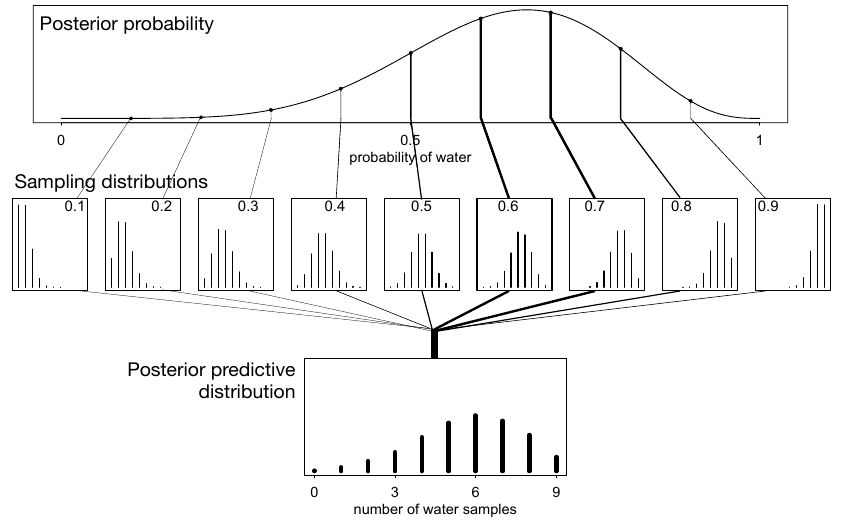
\includegraphics[scale = 0.5]{images/McElreath.png}}
    \caption{Adapted from McElreath.}
\end{figure}

\section{Implementation and Architecture}

\subsection{Object Oriented Programming}

\begin{figure}[H]
    \centerline{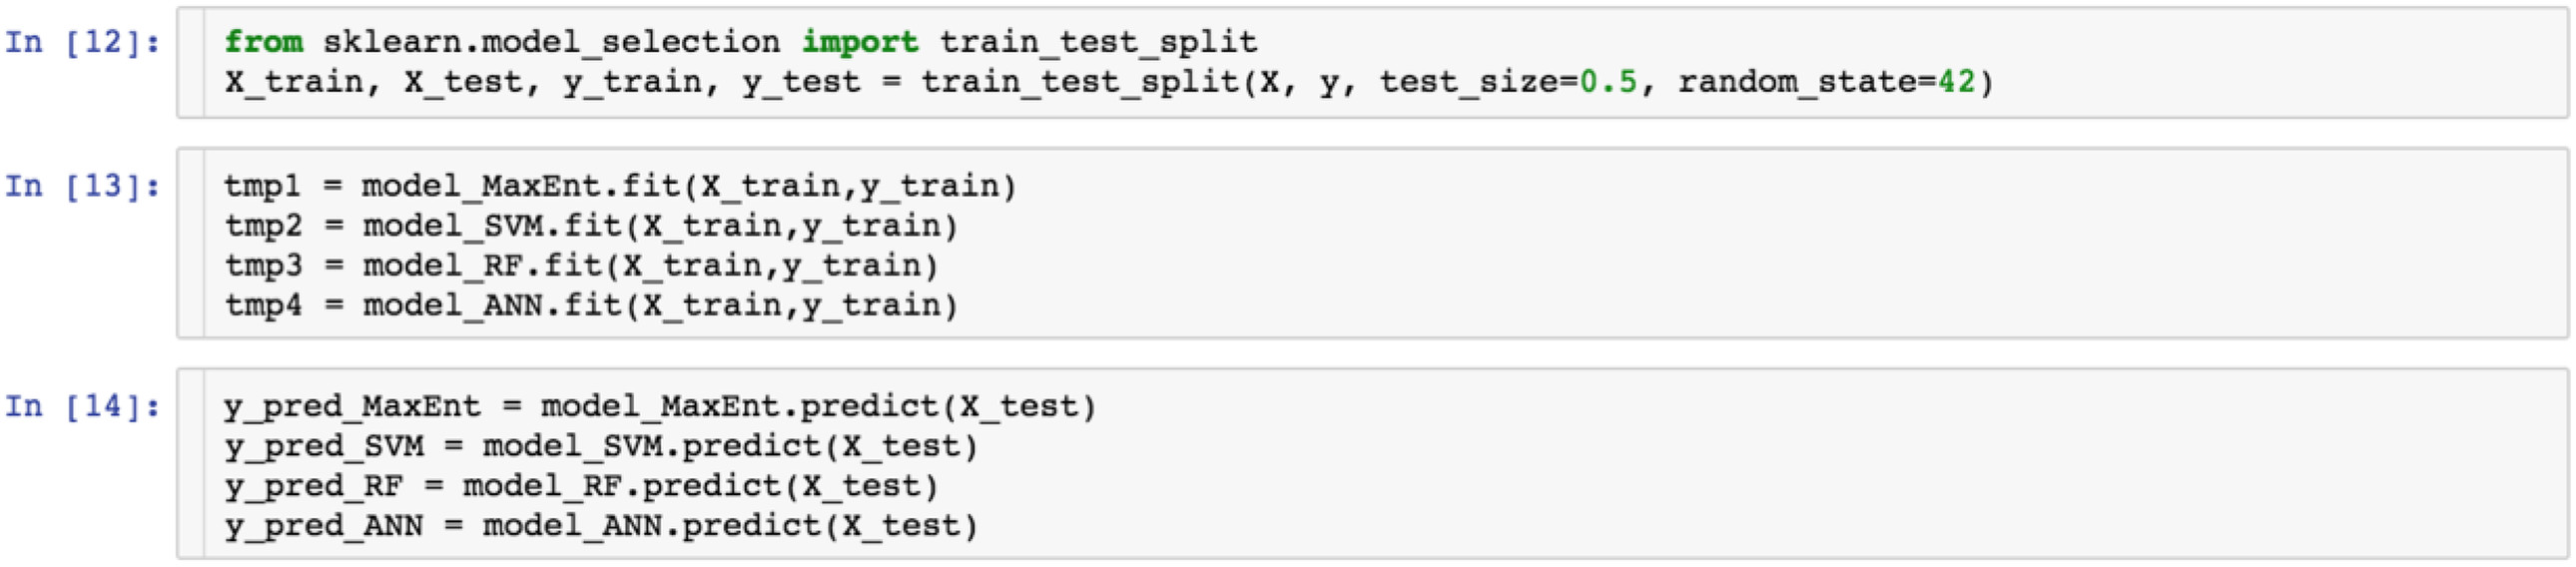
\includegraphics{images/sklearn.jpeg}}
    \caption{Adapted from ... someone. NOTE THIS HAS TO BE WRITTEN AT SOME POINT!!}
\end{figure}

\subsection{Primary Functions}

\begin{lstlisting}[language=Python]
PyCipio.__init__(data, time, values, index = None, split = 0.7):
\end{lstlisting}

\indent \textbf{Description:} 

\indent \indent Initializing the class. Assumes that data is a pandas DataFrame object.

\indent \textbf{Arguments:}

\indent \indent \textit{data (pd.DataFrame):} 

\indent \indent \indent Dataframe containing a column containing time indices and a column containing values. 

\indent \indent \indent Additionally, data can also contain a column which specifies groups in the data, but is not required. 

\indent \indent \textit{time (str):} 

\indent \indent \indent Column name in data, which specifies time indices.

\indent \indent \textit{values (str):} 

\indent \indent \indent Column name in data, which specifies the values of y.
            
\indent \indent \textit{index (str, optional):} 

\indent \indent \indent Column name in data, which specifies a grouping variable. If this variable is given, 

\indent \indent \indent the analysis will be carried out independently for each grouping. Defaults to None.

\indent \indent \textit{split (float, optional):} 

\indent \indent \indent Float indicating the proportion of data used for training. Defaults to 0.7.


\indent \textbf{Example:}
\begin{lstlisting}[language=Python]
		 Pc = PyCipio(data = data, 
                      time = "x", 
                      values = "y", 
                      index = "group", 
                      split = 0.8)

\end{lstlisting}

%%% FUNCTION 2
\hrule

\begin{lstlisting}[language=Python]
    PyCipio.fit(p1, p2, p1_mode, p2_mode, divisor = 20, deviation = 0.2):
\end{lstlisting}

\indent \textbf{Description:} 

\indent \indent Fits the model and plots the prior predictive distribution.

\indent \textbf{Arguments:}

\indent \indent \textit{p1 (tuple):} 

\indent \indent \indent Tuple of integers, where the first value is the value of p and the second value

\indent \indent \indent is the number of components. First value can be specified as a float, 

\indent \indent \indent while the second value must be an integer.

\indent \indent \textit{p2 (tuple):} 

\indent \indent \indent Tuple of integers, where the first value is the value of p and the second value

\indent \indent \indent is the number of components. First value can be specified as a float, 

\indent \indent \indent while the second value must be an integer.

\indent \indent \textit{p1\_mode (str):} 

\indent \indent \indent String indicating whether the seasonal component should be
multiplicative or additive. 

\indent \indent \indent If anything else than "multiplicative" is specified,
the mode defaults to additive.

\indent \indent \textit{p2\_mode (str):} 

\indent \indent \indent String indicating whether the seasonal component should be
multiplicative or additive. 

\indent \indent \indent If anything else than "multiplicative" is specified,
the mode defaults to additive.

\indent \indent \textit{divisor (int, optional):} 

\indent \indent \indent A scaling parameter for adjusting the standard deviation of the distribution
of p. 

\indent \indent \indent The standard deviation of p is set to p/divisor. Defaults to 20. 

\indent \indent \textit{deviation (float, optional):} 

\indent \indent \indent Parameter specifying the standard deviation of the beta for the seasonal
component. Defaults to 0.2.

\indent \textbf{Example:}

\begin{lstlisting}[language=Python]
        Pc.fit(p1 = (7, 2), 
            p2 = (365.25, 2), 
            p1_mode = "additive", 
            p2_mode = "multiplicative", 
            divisor = 15, 
            deviation = 0.3)    
\end{lstlisting}

%%% FUNCTION 3

\hrule

\begin{lstlisting}[language=Python]
    PyCipio.sample_mod(posterior_draws = 2000, post_pred_draws = 1000, 
    prior_pred_draws = 1000, random_seed = 42, chains = 2):
\end{lstlisting}

\indent \textbf{Description:} 

\indent \indent Sample the posterior, the posterior predictive, the prior predictive distribution and generate 

\indent \indent predictions on the test data.

\indent \textbf{Arguments:}

\indent \indent \textit{posterior\_draws (int, optional):} 

\indent \indent \indent Number of draws for the posterior. Defaults to 2000.

\indent \indent \textit{prior\_pred\_draws (int, optional):} 

\indent \indent \indent Number of draws for the prior predictive distribution. Defaults to 1000.

\indent \indent \textit{random\_seed (int, optional):}

\indent \indent \indent Random seed for ensuring reproducibility. Defaults to 42.

\indent \indent \textit{chains (int, optional):} 

\indent \indent \indent Number of chains used for sampling the posterior. Defaults to 2.

\indent \textbf{Example:}

\begin{lstlisting}[language=Python]
        Pc.sample_mod(posterior_draws = 3000, 
        post_pred_draws = 1500, 
        prior_pred_draws = 1500, 
        random_seed = 13, 
        chains = 4)
\end{lstlisting}

%%% FUNCTION 4

\hrule

\begin{lstlisting}[language=Python]
    PyCipio.plot_fit_idx(idx = None, path = False):
\end{lstlisting}

\indent \textbf{Description:} 

\indent \indent Plots the posterior predictive distribution overlayed on the training data.

\indent \textbf{Arguments:}

\indent \indent \textit{idx (list, optional):} 

\indent \indent \indent List of strings containing the names of the groups to plot. Defaults to None.

\indent \indent \textit{path (str, optional):}

\indent \indent \indent String specifying the path for saving the plot. 

\indent \indent \indent File-extension is automatically inserted and is hard set to .png. Defaults to False.

\indent \textbf{Example:}

\begin{lstlisting}[language=Python]
        Pc.plot_fit_idx(idx = ["group1", "group2"], path = "my_path/my_plot")
\end{lstlisting}

\noindent \textbf{Note:}

\noindent The same functionality exists for plotting the posterior predictive distribution overlayed on the training data. This method called \textit{plot\_prediction\_idx} is identical in inputs and outputs, but only differs on this point. For more details, see the full docstrings on Github. 

%%% FUNCTION 5

\hrule

\begin{lstlisting}[language=Python]
    PyCipio.plot_residuals(idx = None, path = False):
\end{lstlisting}

\indent \textbf{Description:} 

\indent \indent Plots the residuals from predictions generated by the model.

\indent \textbf{Arguments:}

\indent \indent \textit{idx (list, optional):}

\indent \indent \indent List of strings containing the names of the groups to plot. Defaults to None.

\indent \indent \textit{path (str, optional):}

\indent \indent \indent String specifying the path for saving the plot. 

\indent \indent \indent File-extension is automatically inserted and is hard set to .png. Defaults to False.

\indent \textbf{Example:}

\begin{lstlisting}[language=Python]
        Pc.plot_residuals(idx = ["group1", "group2"], path = "my_path/my_plot")
\end{lstlisting}

\subsection{Workflow}

\begin{figure}[H]
    \centerline{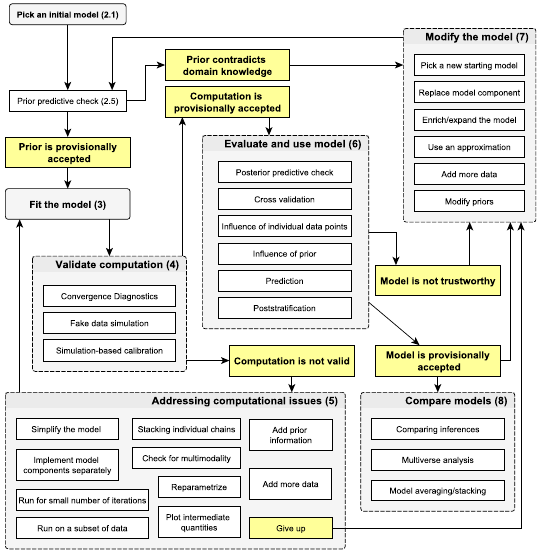
\includegraphics[scale = 0.5]{images/Gelman.png}}
    \caption{Adapted from Gelman}
\end{figure}

\begin{lstlisting}[language=Python, caption=]
    #prep data (pandas dataframe containing a time series)
    d = pd.DataFrame(data)
    
    ##### create class ######
    Pc = pc.PyCipio(d, time = "time_column", 
                    values = "y_values", 
                    index = "idx_column", 
                    split = 0.7)
    
    ##### fit model: 
    Pc.fit(p1 = (7, 1), p2 = (30, 1), p1_mode = "multiplicative", p2_mode = "additive")
    
    ##### sample #####
    Pc.sample_mod()
    
    ##### plotting #####
    Pc.plot_trace()
    Pc.plot_pp()
    
    ### plot training ###
    Pc.plot_fit_idx(idx = ["group 1", "group 2"])
    
    ### plot predict ###
    Pc.plot_predict_idx(idx = ["group 1", "group 2"])
    
    ### get errors ###
    Pc.get_errors()
    
    ### plot residuals ###
    Pc.plot_residuals(idx = ["group 1", "group 2"])
    
    ### save idata ### - This is if you want to save your model for later use
    Pc.save_idata()
\end{lstlisting}

\section{Related work and differences}

\subsection{fpp3}

\subsection{Facebook Prophet}

\section{Examples}

\subsection{Example 1}

\begin{figure}[H]
    \centerline{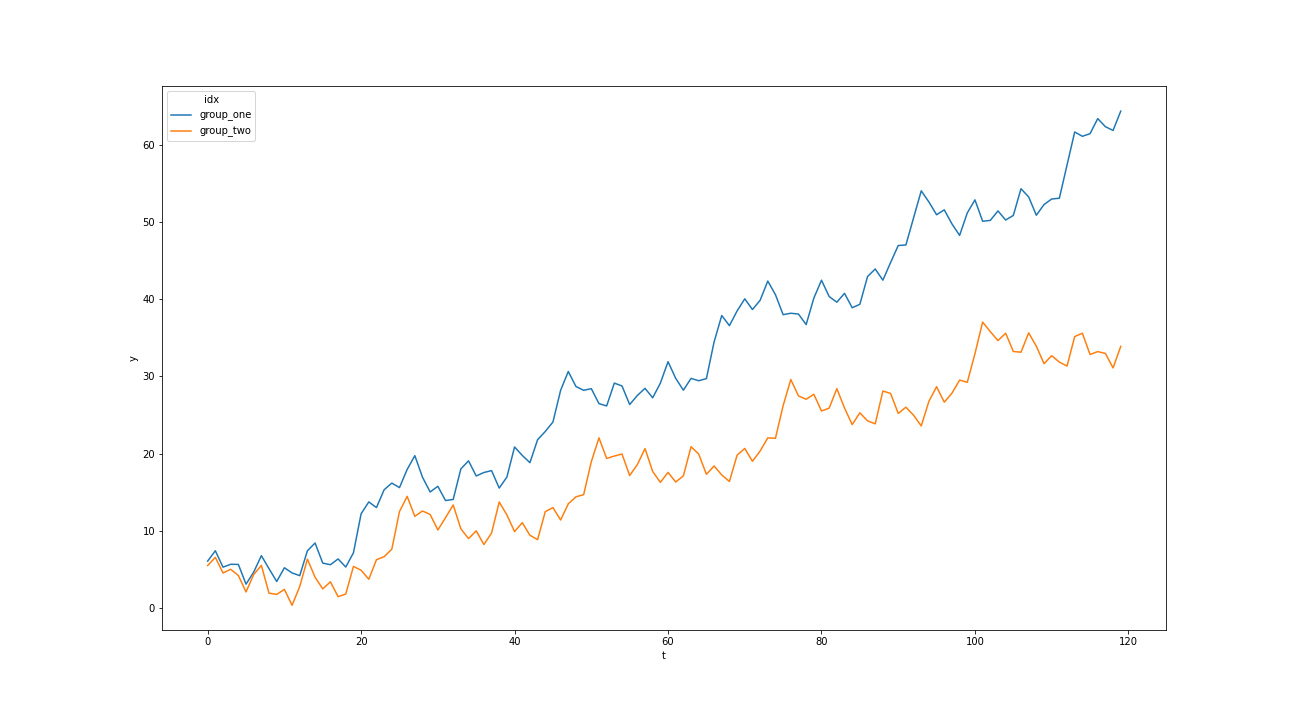
\includegraphics[scale = 0.45]{../plots/ex1_plot_data.png}}
    \caption{Lineplot of the two simulated time-series}
\end{figure}


Obviously here you write something, Obviously here you write something, Obviously here you write something, Obviously here you write something, Obviously here you write something, Obviously here you write something, Obviously here you write something, Obviously here you write something, Obviously here you write something, Obviously here you write something, Obviously here you write something, Obviously here you write something, Obviously here you write something, Obviously here you write something, Obviously here you write something, 

\begin{figure}[ht]
    \centering
    \subfigure[First plot]{%
        \label{fig:supfigure1}
        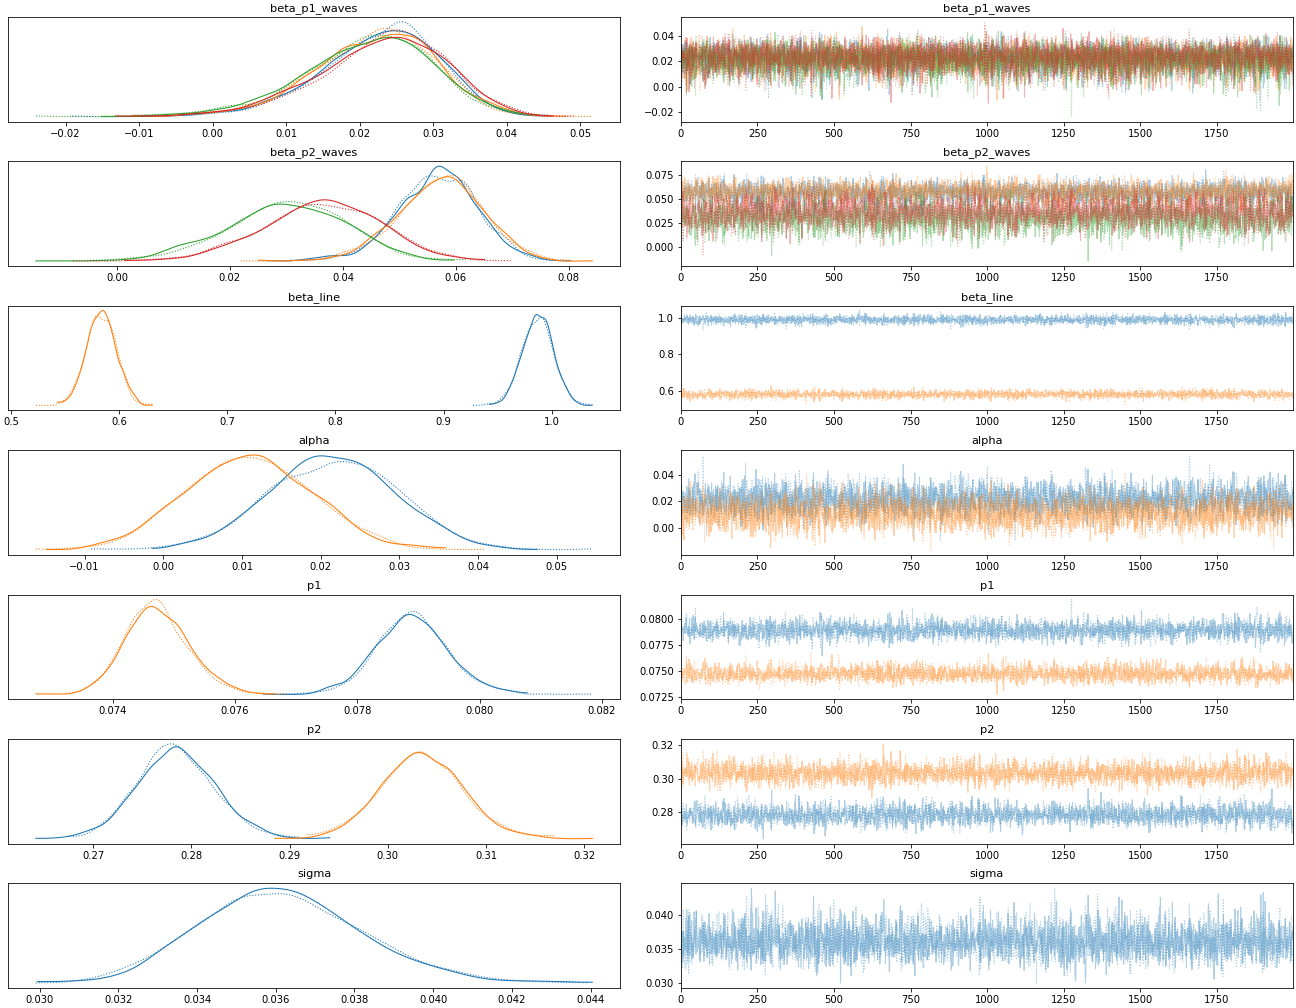
\includegraphics[width = 0.30 \textwidth]{../plots/ex1_first_plot_trace.png}}
    \quad
    \subfigure[Second plot]{%
        \label{fig:supfigure2}
        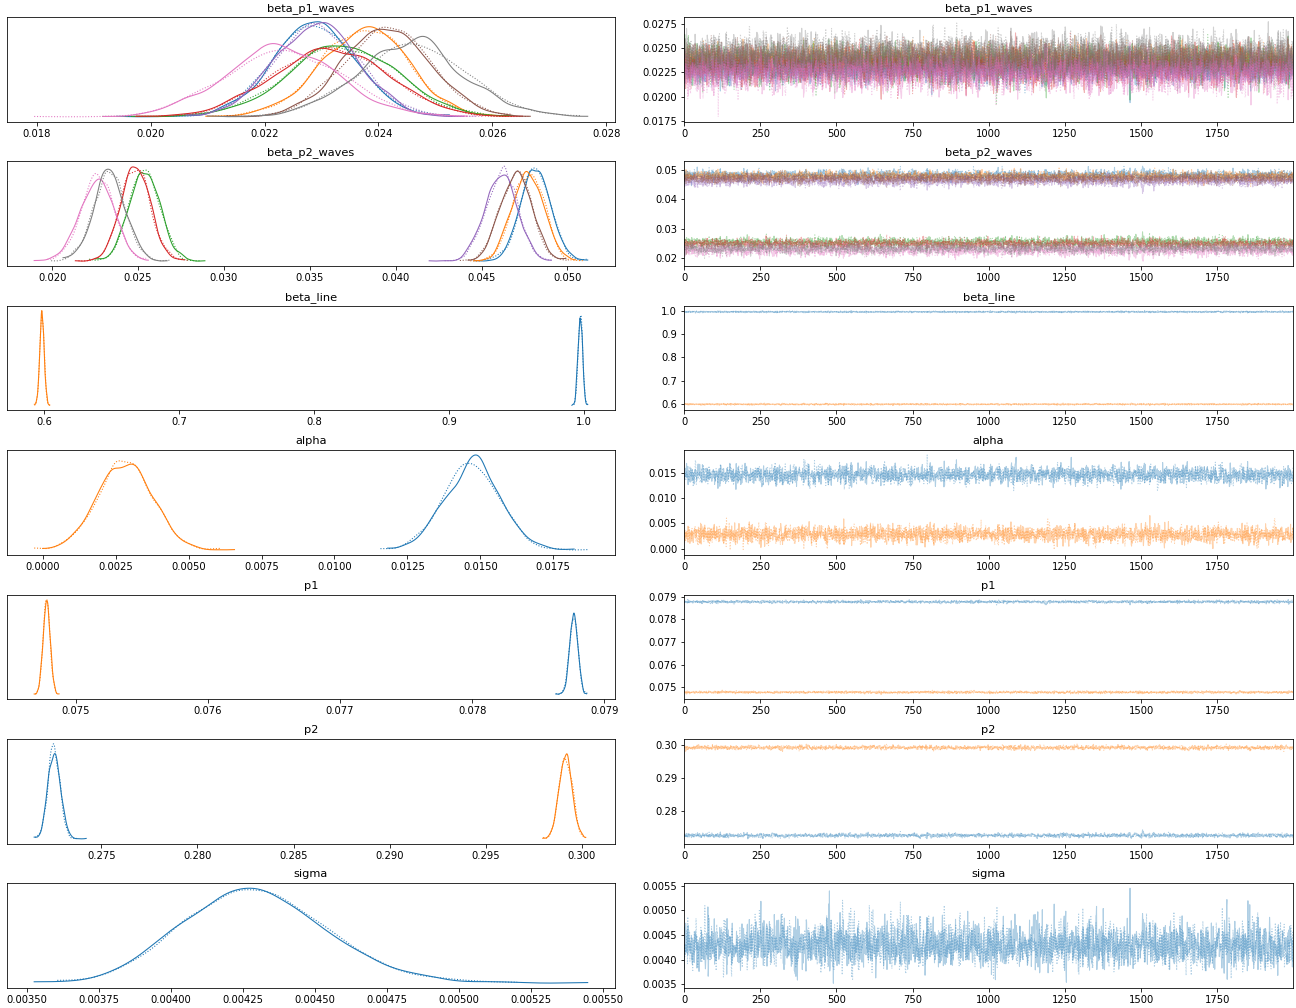
\includegraphics[width = 0.30 \textwidth]{../plots/ex1_second_plot_trace.png}}
    \subfigure[Third Plot]{%
        \label{fig:supfigure3}
        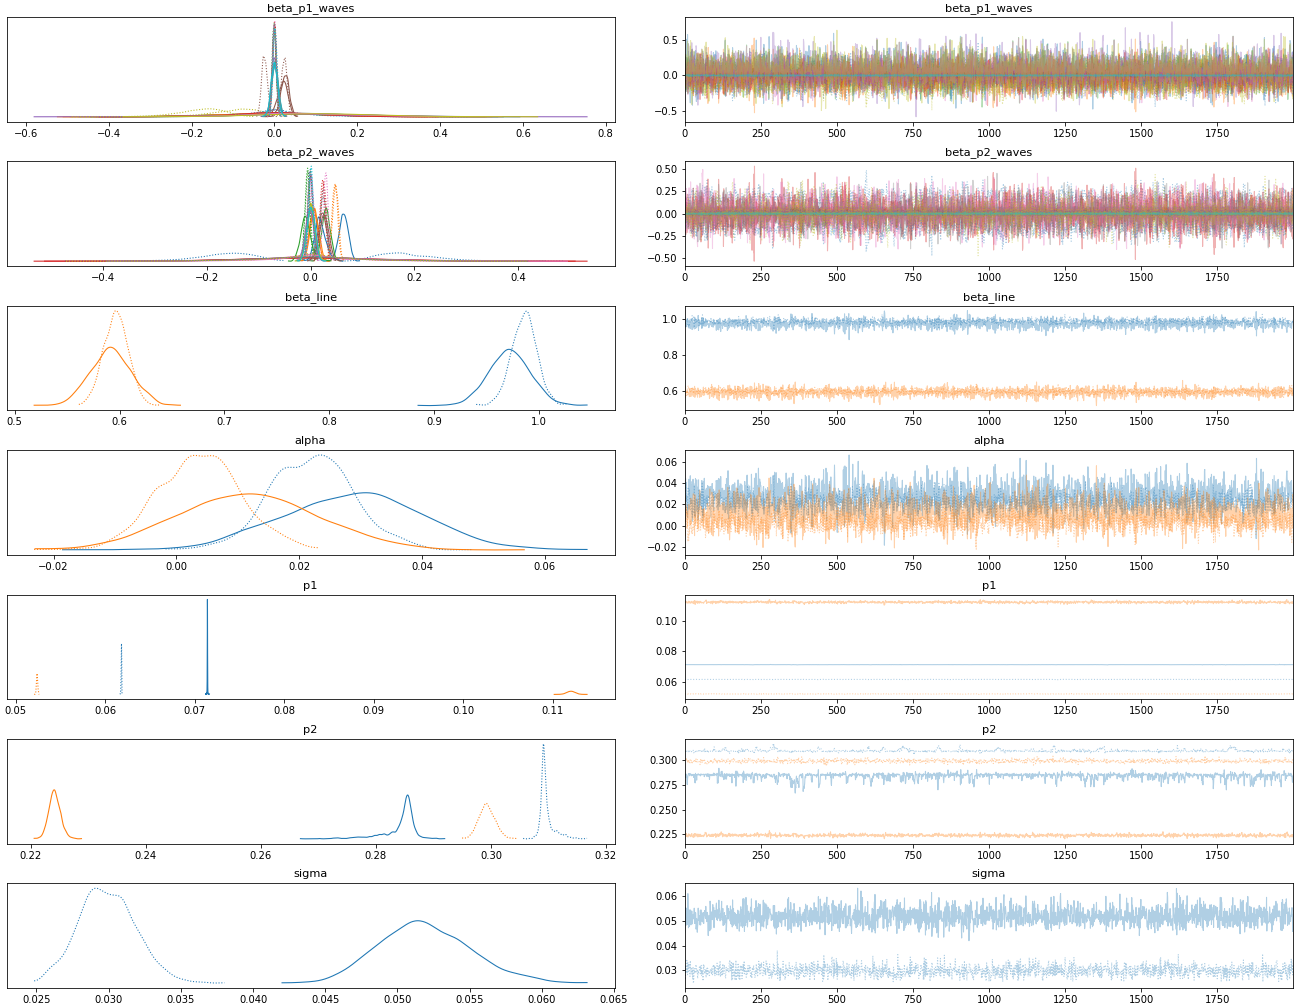
\includegraphics[width = 0.30 \textwidth]{../plots/ex1_third_plot_trace.png}}
    \quad
    \caption{Predictions in one and 2 groups}
\end{figure}

Obviously here you write something, Obviously here you write something, Obviously here you write something, Obviously here you write something, Obviously here you write something, Obviously here you write something, Obviously here you write something, Obviously here you write something, 

\begin{figure}[ht]
    \centering
    \subfigure[First plot]{%
        \label{fig:supfigure1}
        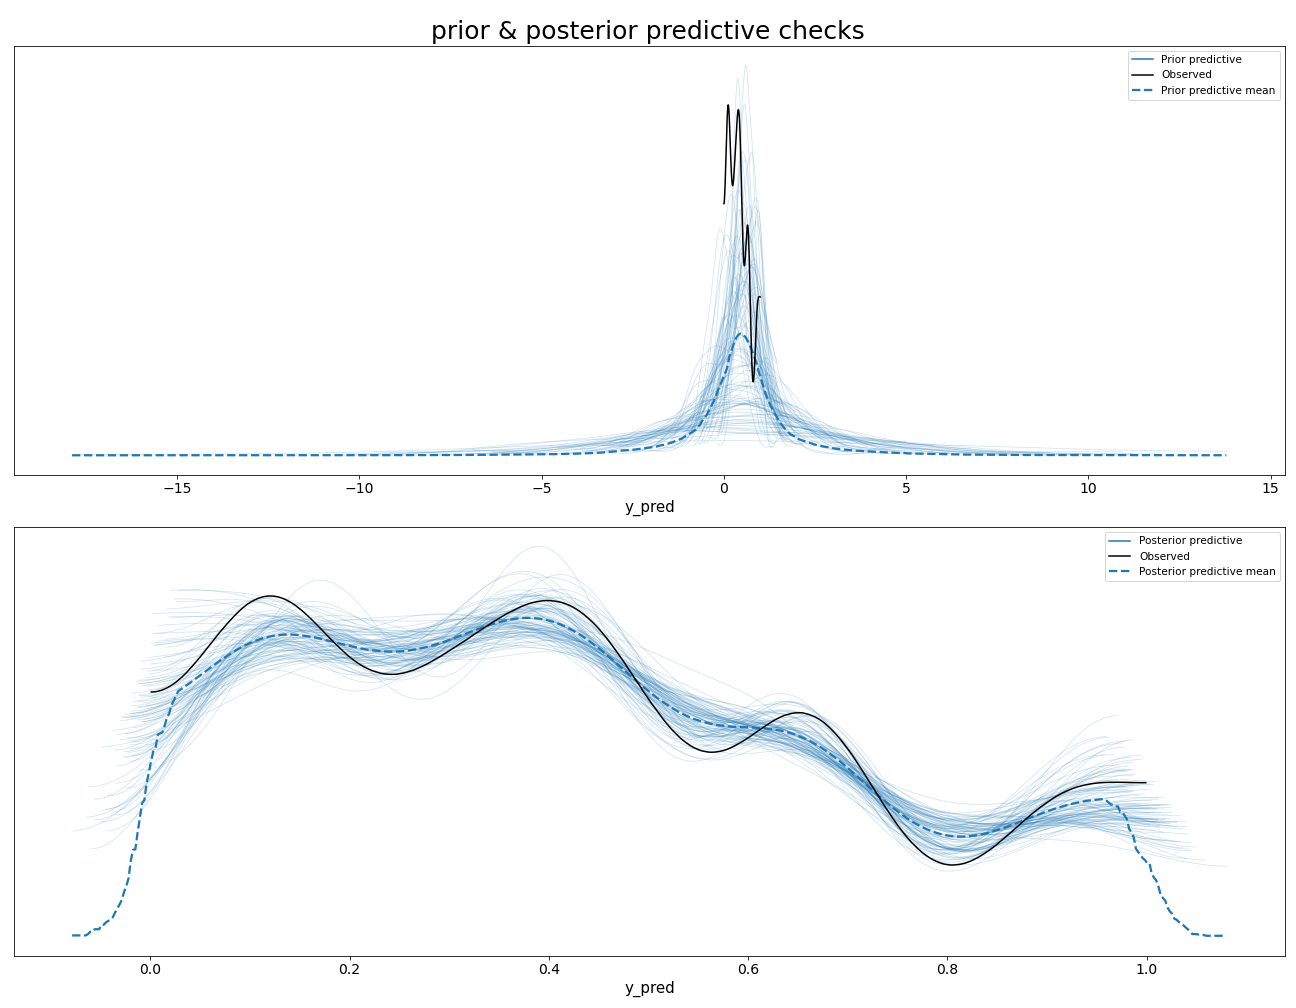
\includegraphics[width = 0.30 \textwidth]{../plots/ex1_first_plot_pp.png}}
    \quad
    \subfigure[Second plot]{%
        \label{fig:supfigure2}
        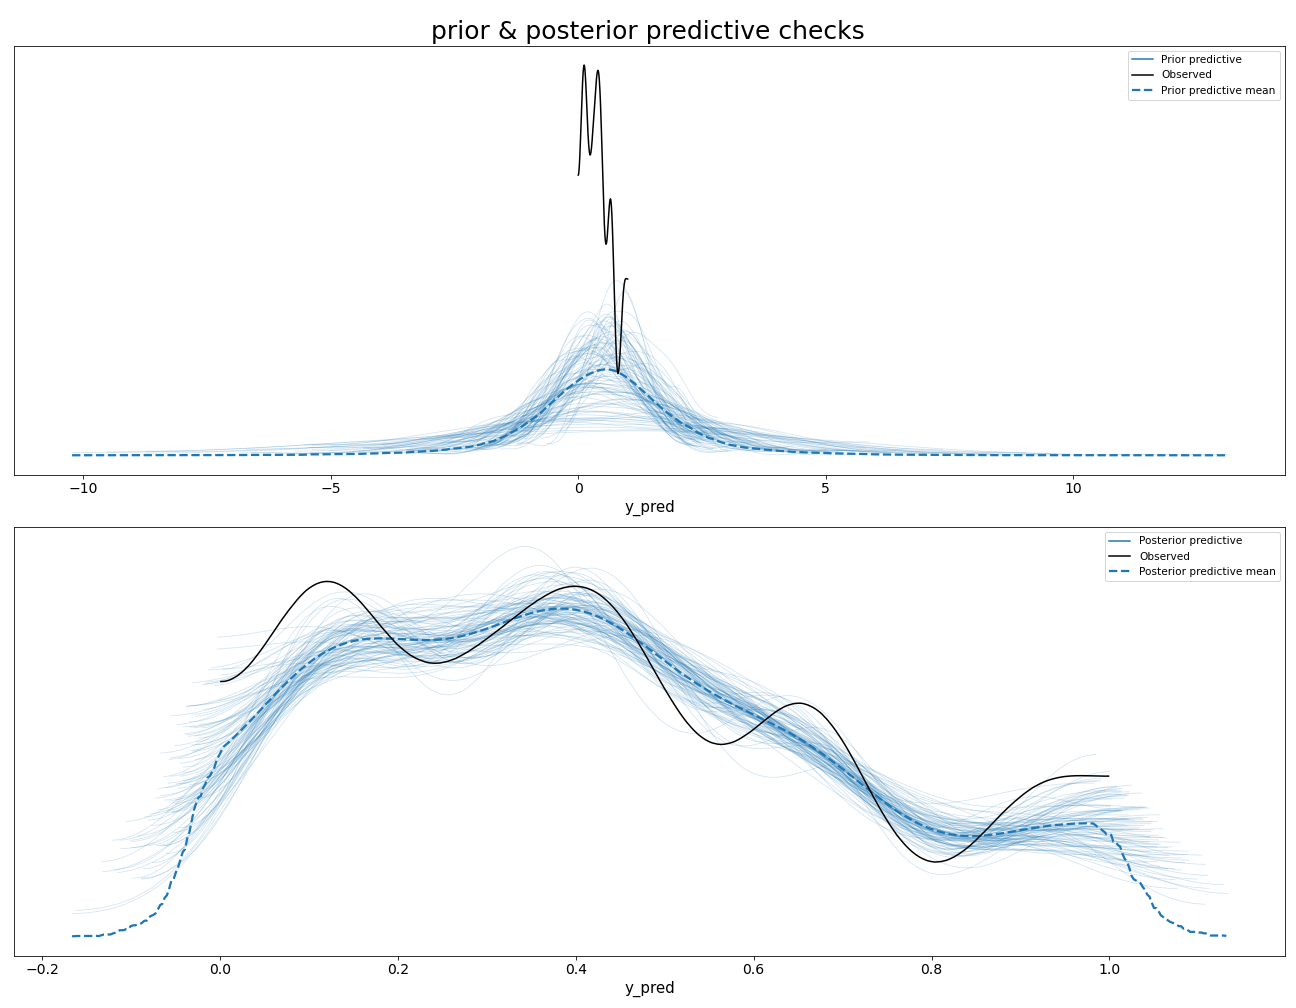
\includegraphics[width = 0.30 \textwidth]{../plots/ex1_second_plot_pp.png}}
    \subfigure[Third Plot]{%
        \label{fig:supfigure3}
        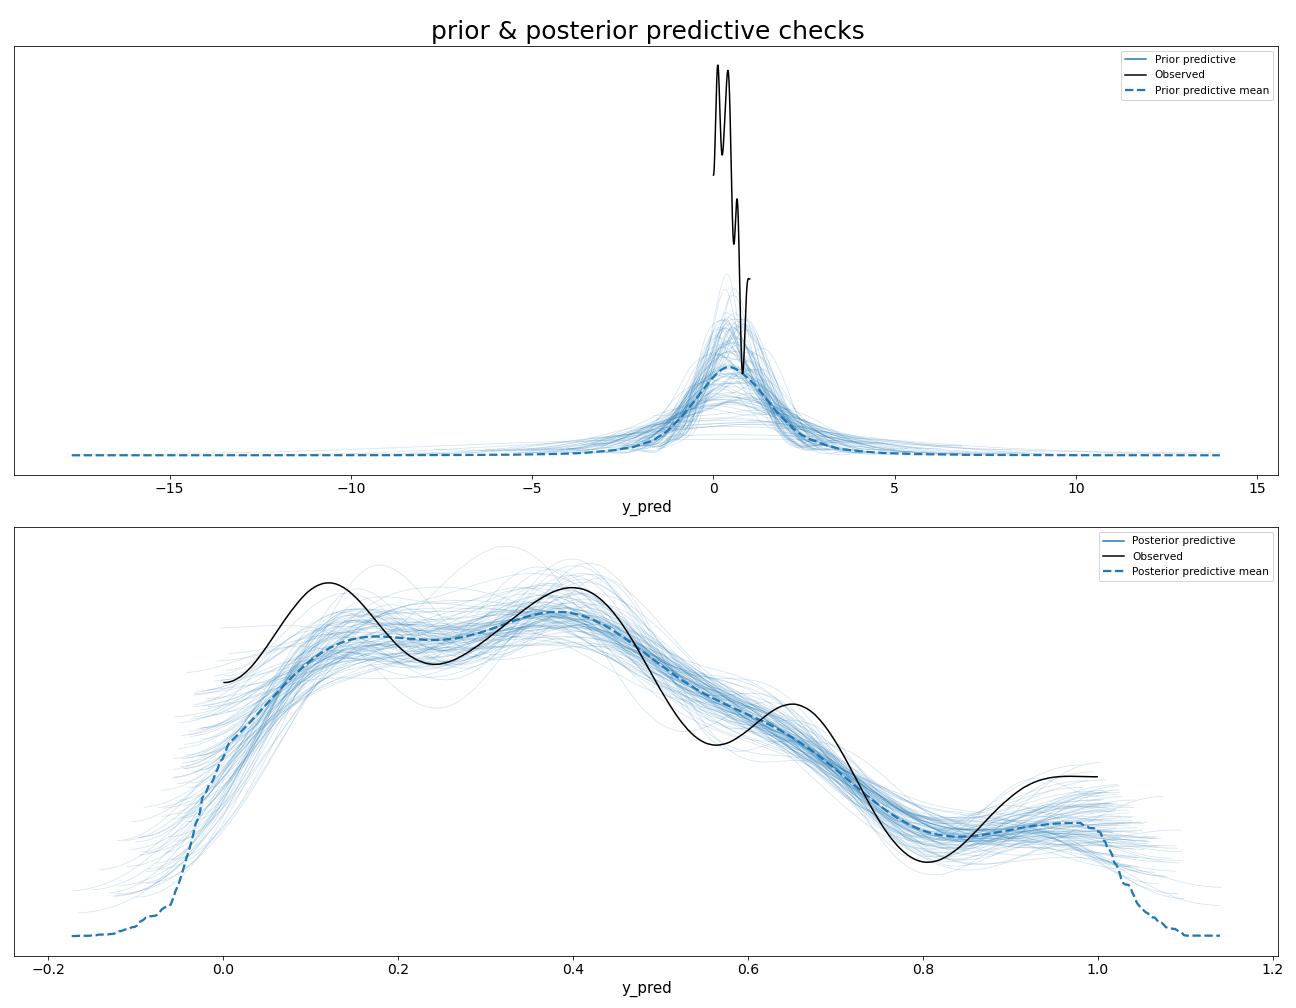
\includegraphics[width = 0.30 \textwidth]{../plots/ex1_third_plot_pp.png}}
    \quad
    \caption{Predictions in one and 2 groups}
\end{figure}

Obviously here you write something, Obviously here you write something, Obviously here you write something, Obviously here you write something, Obviously here you write something, Obviously here you write something, Obviously here you write something, 

\begin{figure}[ht]
    \centering
    \subfigure[First plot]{%
        \label{fig:supfigure1}
        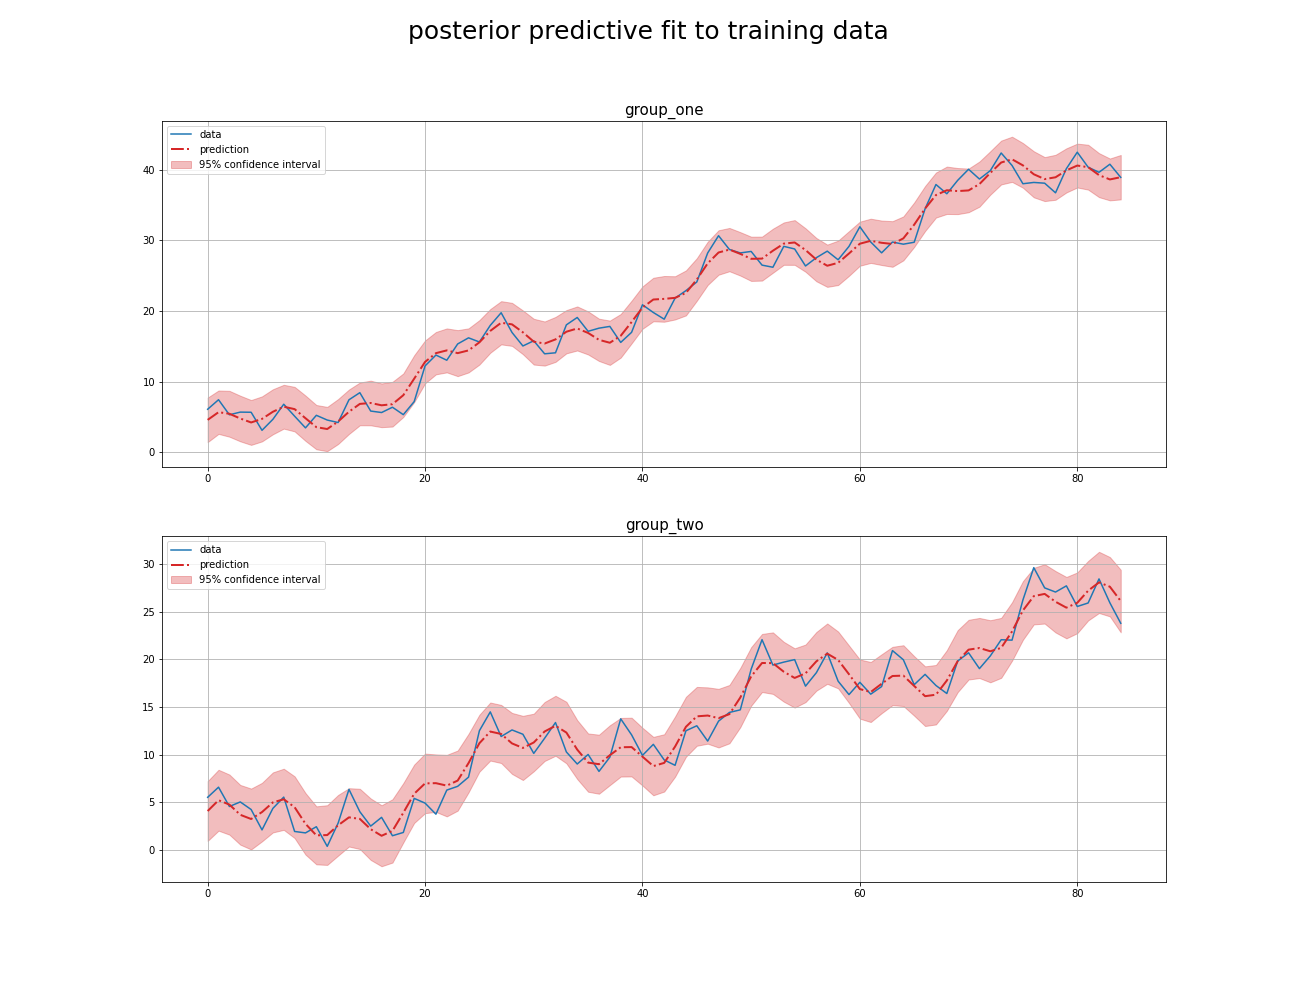
\includegraphics[width = 0.30 \textwidth]{../plots/ex1_first_plot_fit_idx_all.png}}
    \quad
    \subfigure[Second plot]{%
        \label{fig:supfigure2}
        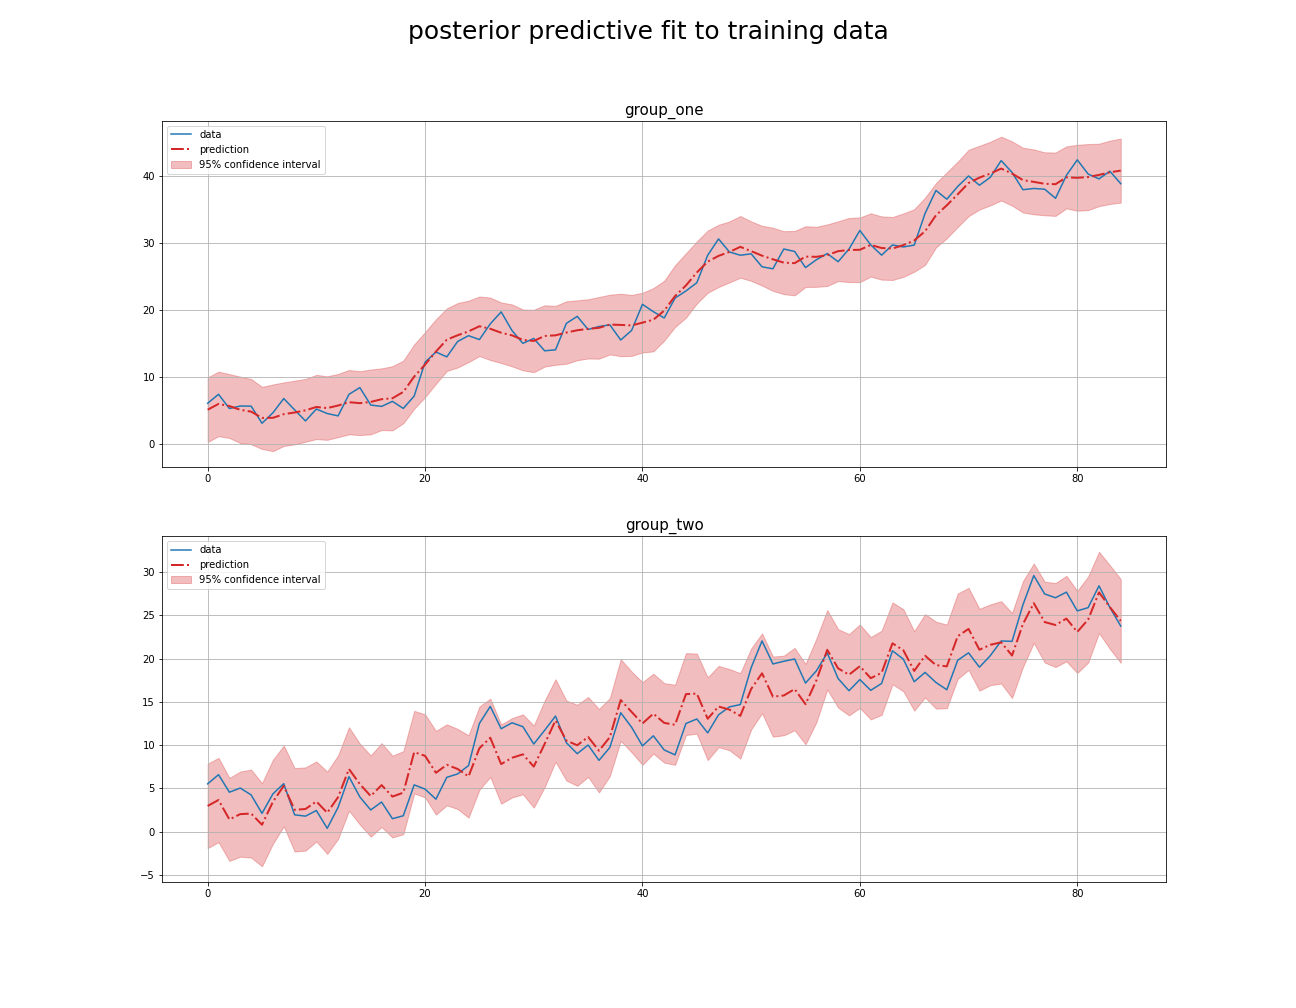
\includegraphics[width = 0.30 \textwidth]{../plots/ex1_second_plot_fit_idx_all.png}}
    \subfigure[Third Plot]{%
        \label{fig:supfigure3}
        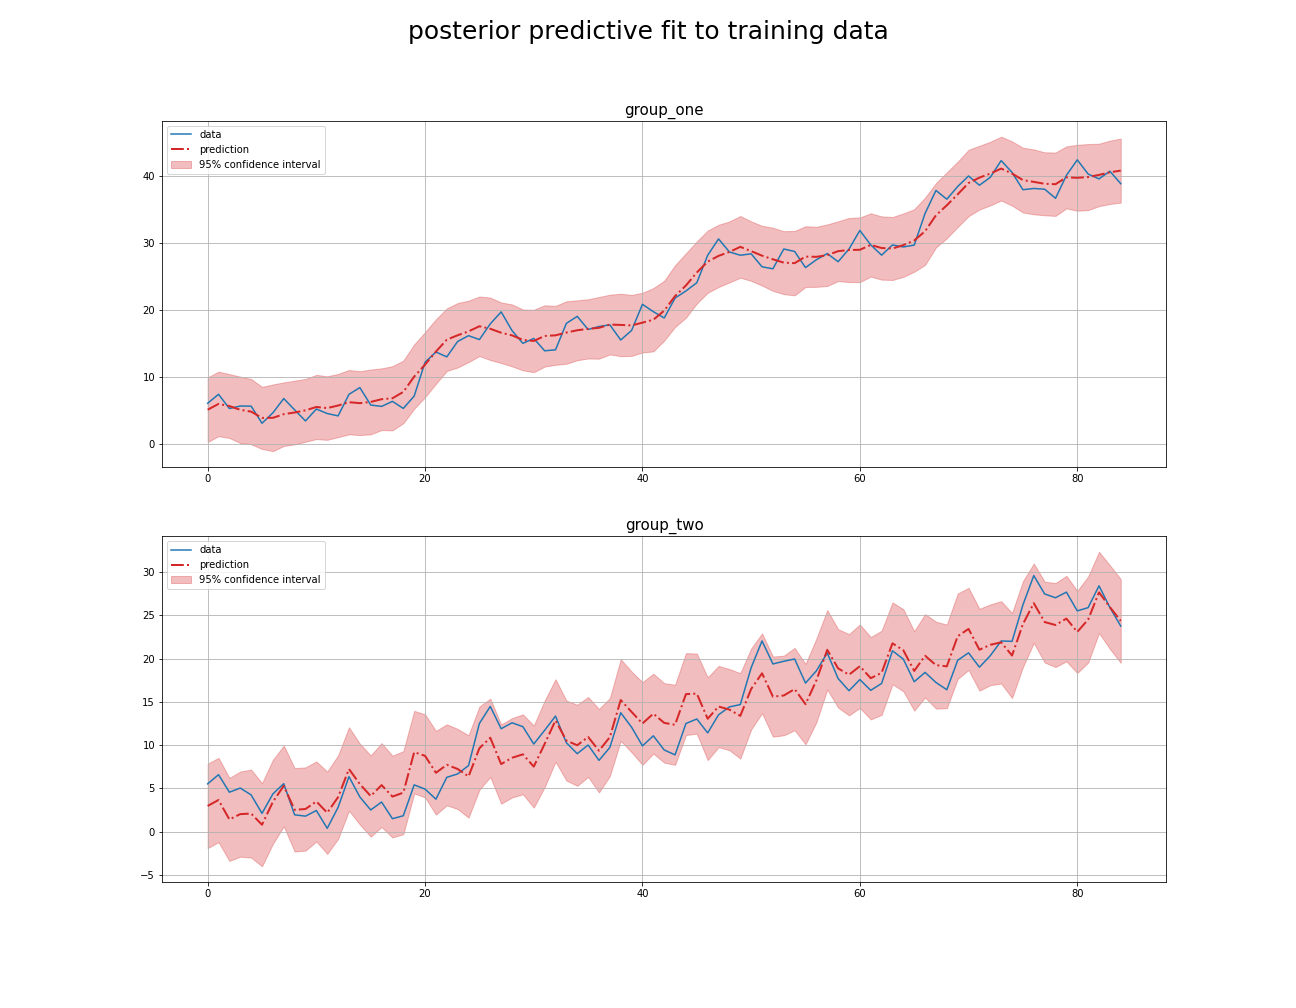
\includegraphics[width = 0.30 \textwidth]{../plots/ex1_third_plot_fit_idx_all.png}}
    \quad
    \caption{Predictions in one and 2 groups}
\end{figure}

Obviously here you write something, Obviously here you write something, Obviously here you write something, Obviously here you write something, Obviously here you write something, Obviously here you write something, Obviously here you write something, 

\begin{figure}[H]
    \centering
    \subfigure[First plot]{%
        \label{fig:supfigure1}
        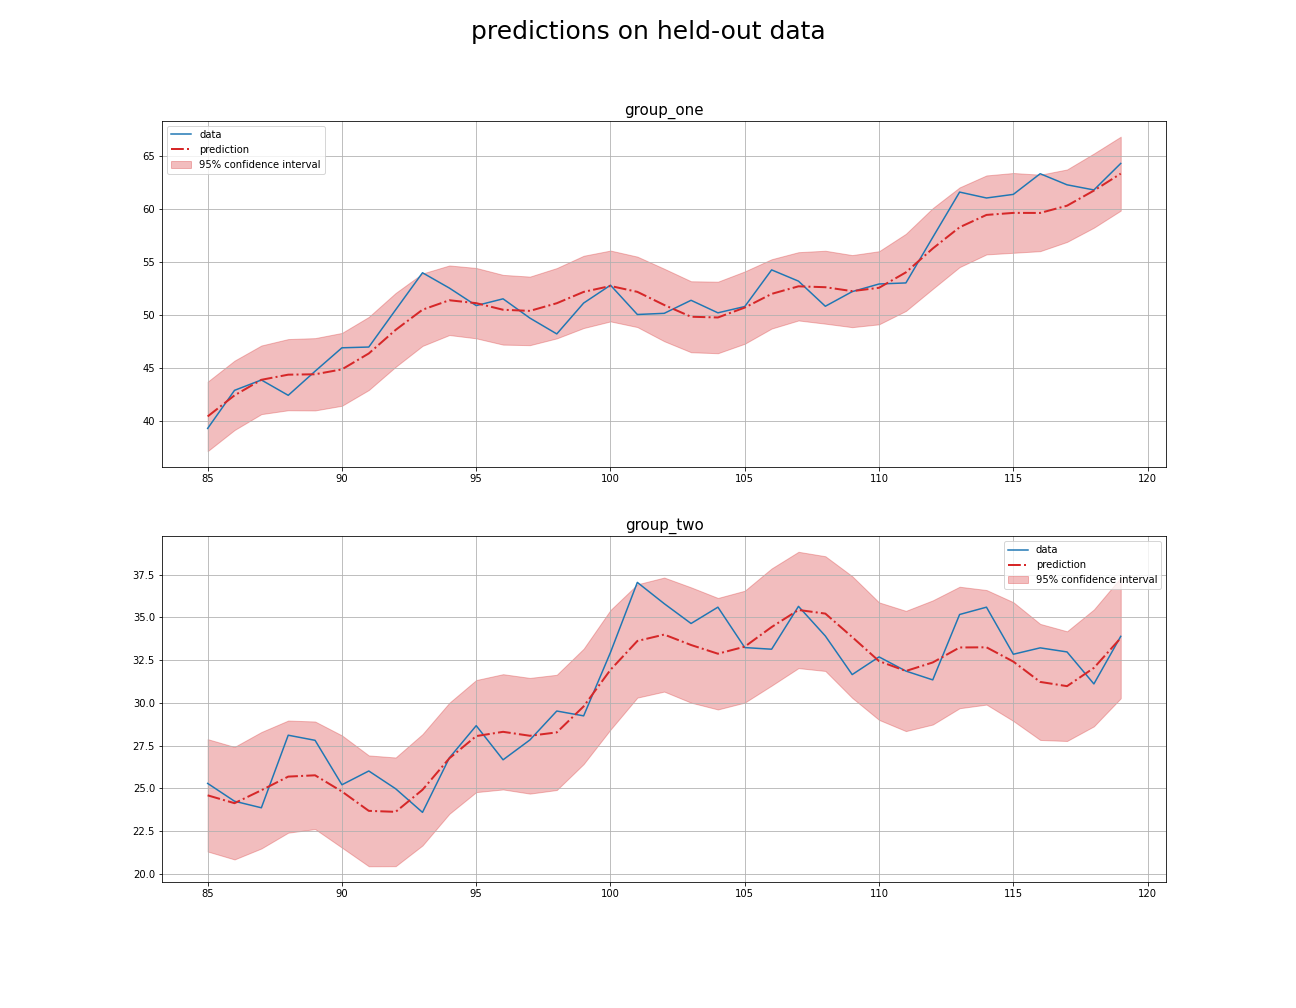
\includegraphics[width = 0.45 \textwidth]{../plots/ex1_first_plot_predict_idx_all.png}}
    \quad
    \subfigure[Second plot]{%
        \label{fig:supfigure2}
        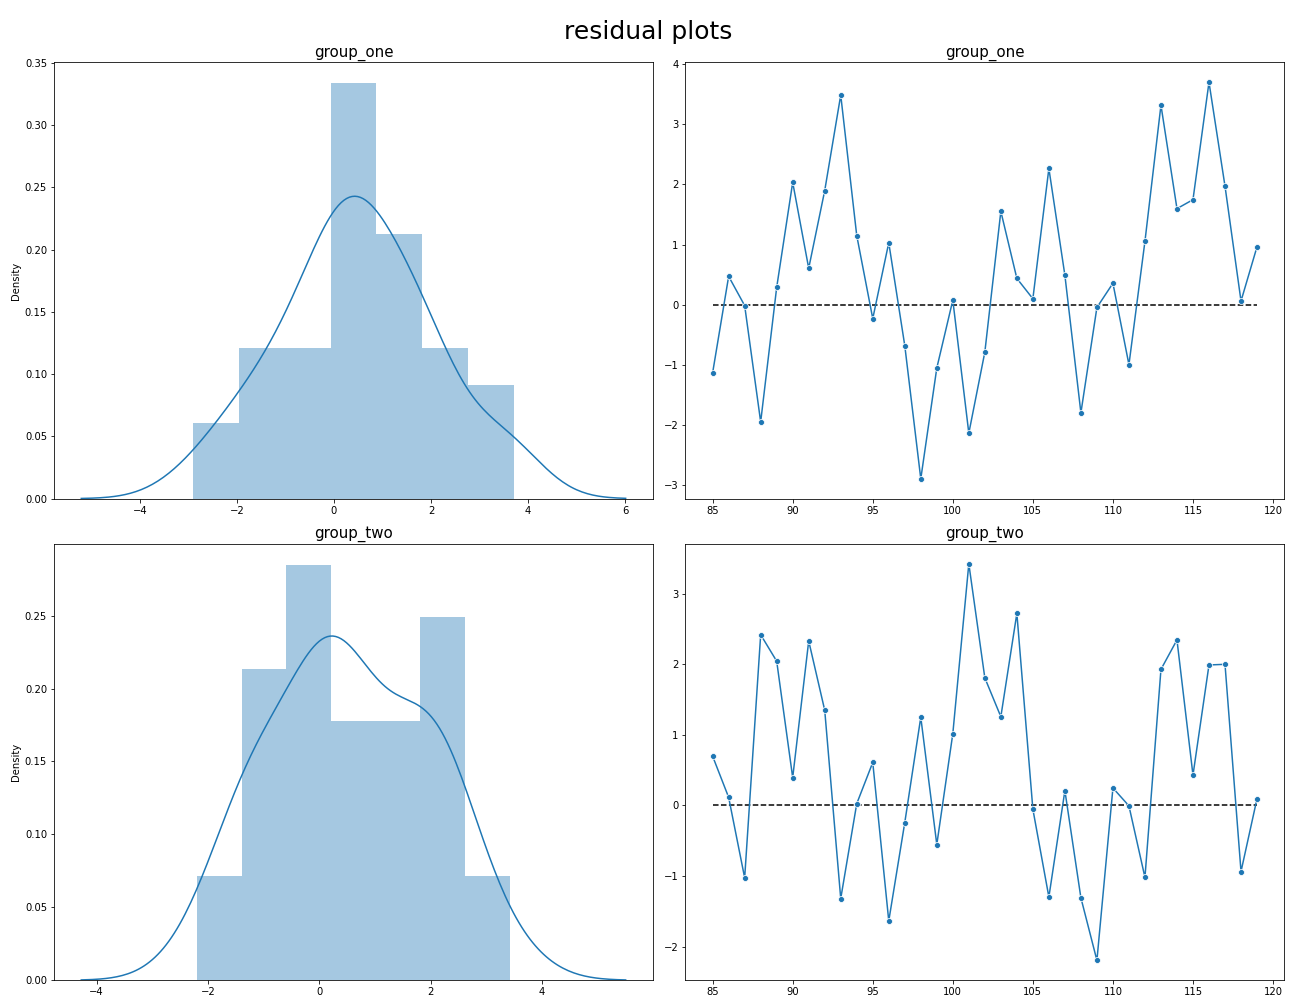
\includegraphics[width = 0.45 \textwidth]{../plots/ex1_first_residual_plots_all.png}}
    \subfigure[Third Plot]{%
        \label{fig:supfigure3}
        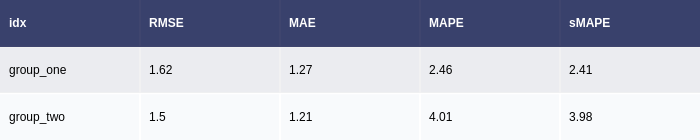
\includegraphics[width = 0.75 \textwidth]{../plots/ex1_first_get_errors.png}}
    \quad
    \caption{Predictions in one and 2 groups}
\end{figure}
\begin{figure}[H]
    \centering
    \subfigure[First plot]{%
        \label{fig:supfigure1}
        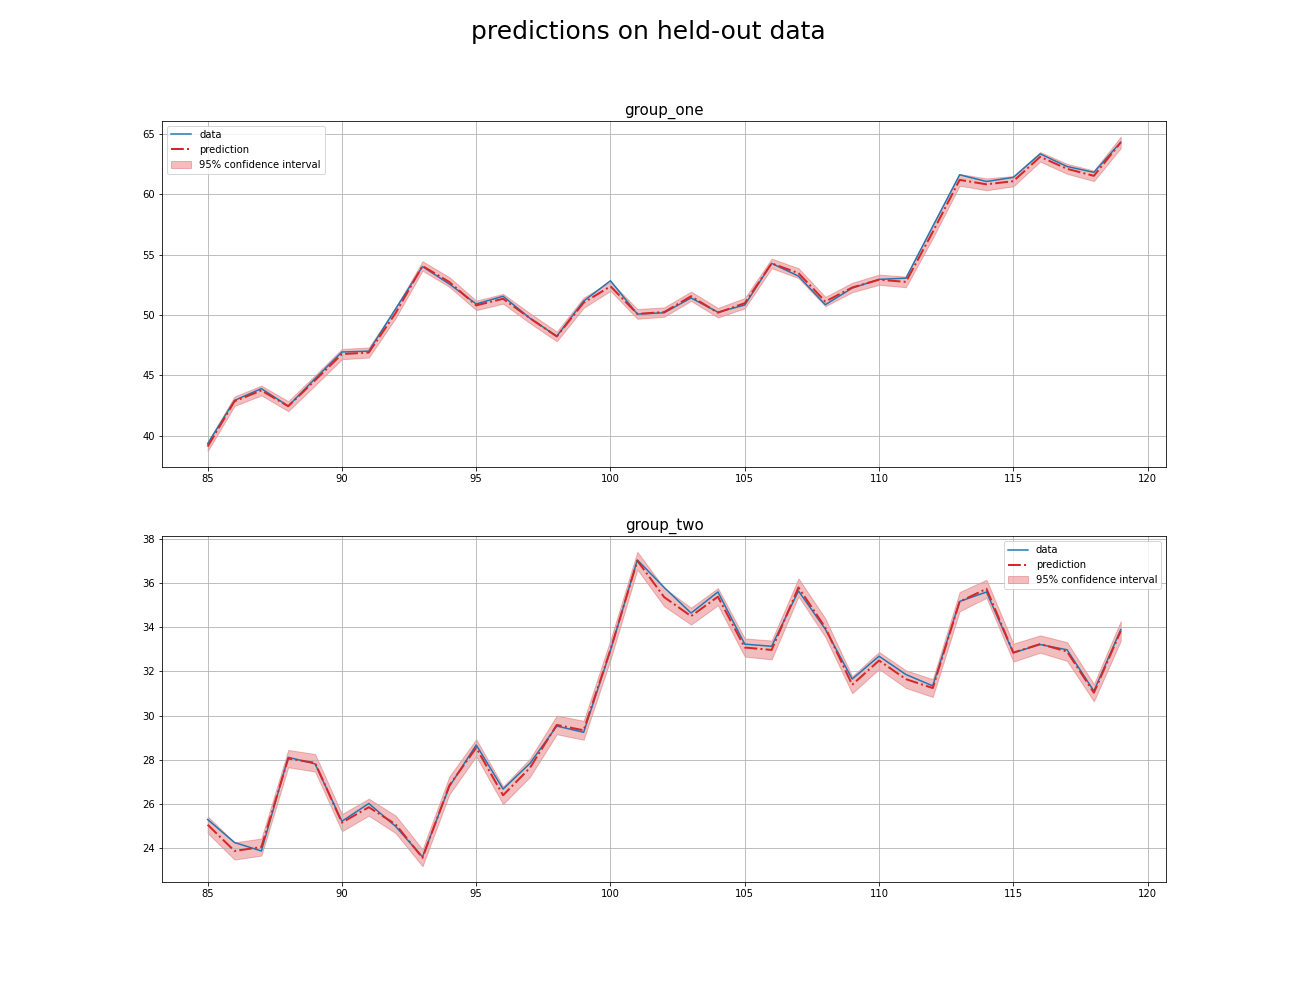
\includegraphics[width = 0.45 \textwidth]{../plots/ex1_second_plot_predict_idx_all.png}}
    \quad
    \subfigure[Second plot]{%
        \label{fig:supfigure2}
        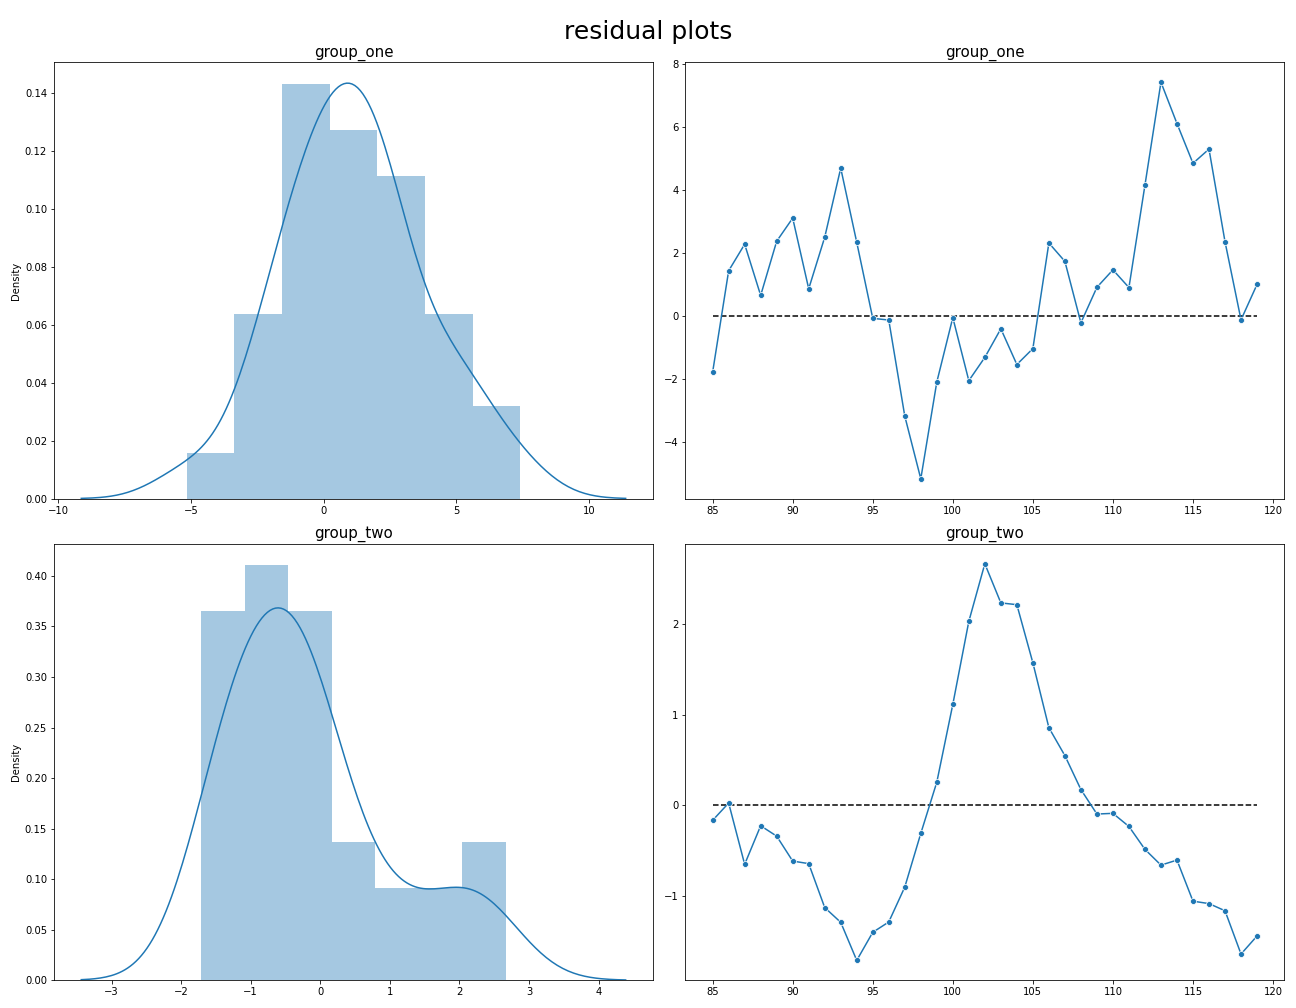
\includegraphics[width = 0.45 \textwidth]{../plots/ex1_second_residual_plots_all.png}}
    \subfigure[Third Plot]{%
        \label{fig:supfigure3}
        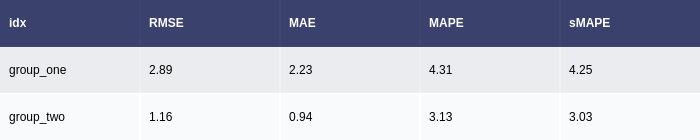
\includegraphics[width = 0.75 \textwidth]{../plots/ex1_second_get_errors.png}}
    \quad
    \caption{Predictions in one and 2 groups}
\end{figure}

Obviously here you write something, Obviously here you write something, Obviously here you write something, Obviously here you write something, Obviously here you write something, Obviously here you write something, 

\begin{figure}[H]
    \centering
    \subfigure[First plot]{%
        \label{fig:supfigure1}
        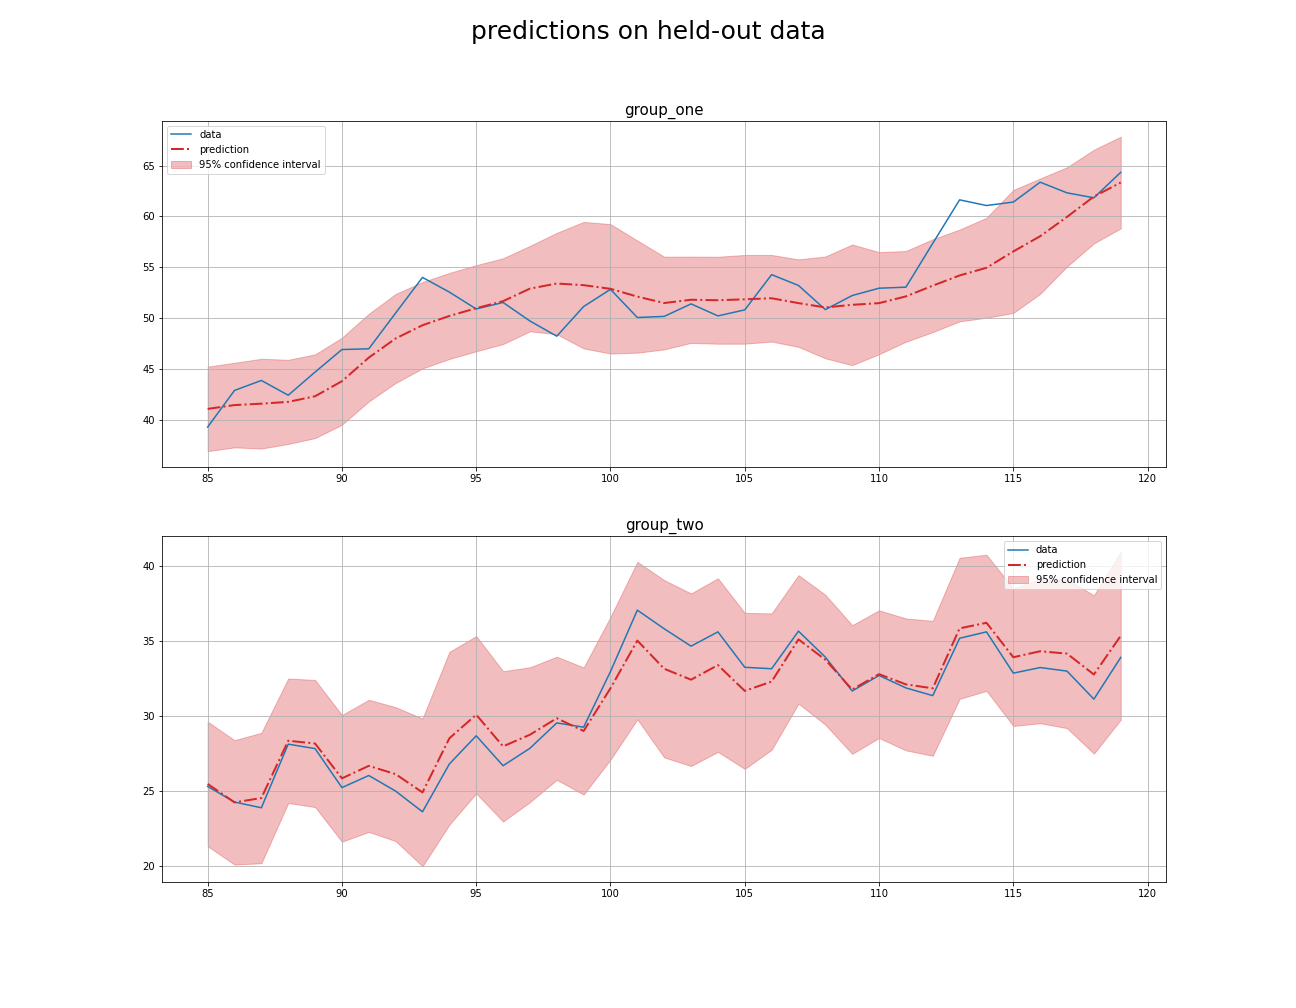
\includegraphics[width = 0.45 \textwidth]{../plots/ex1_third_plot_predict_idx_all.png}}
    \quad
    \subfigure[Second plot]{%
        \label{fig:supfigure2}
        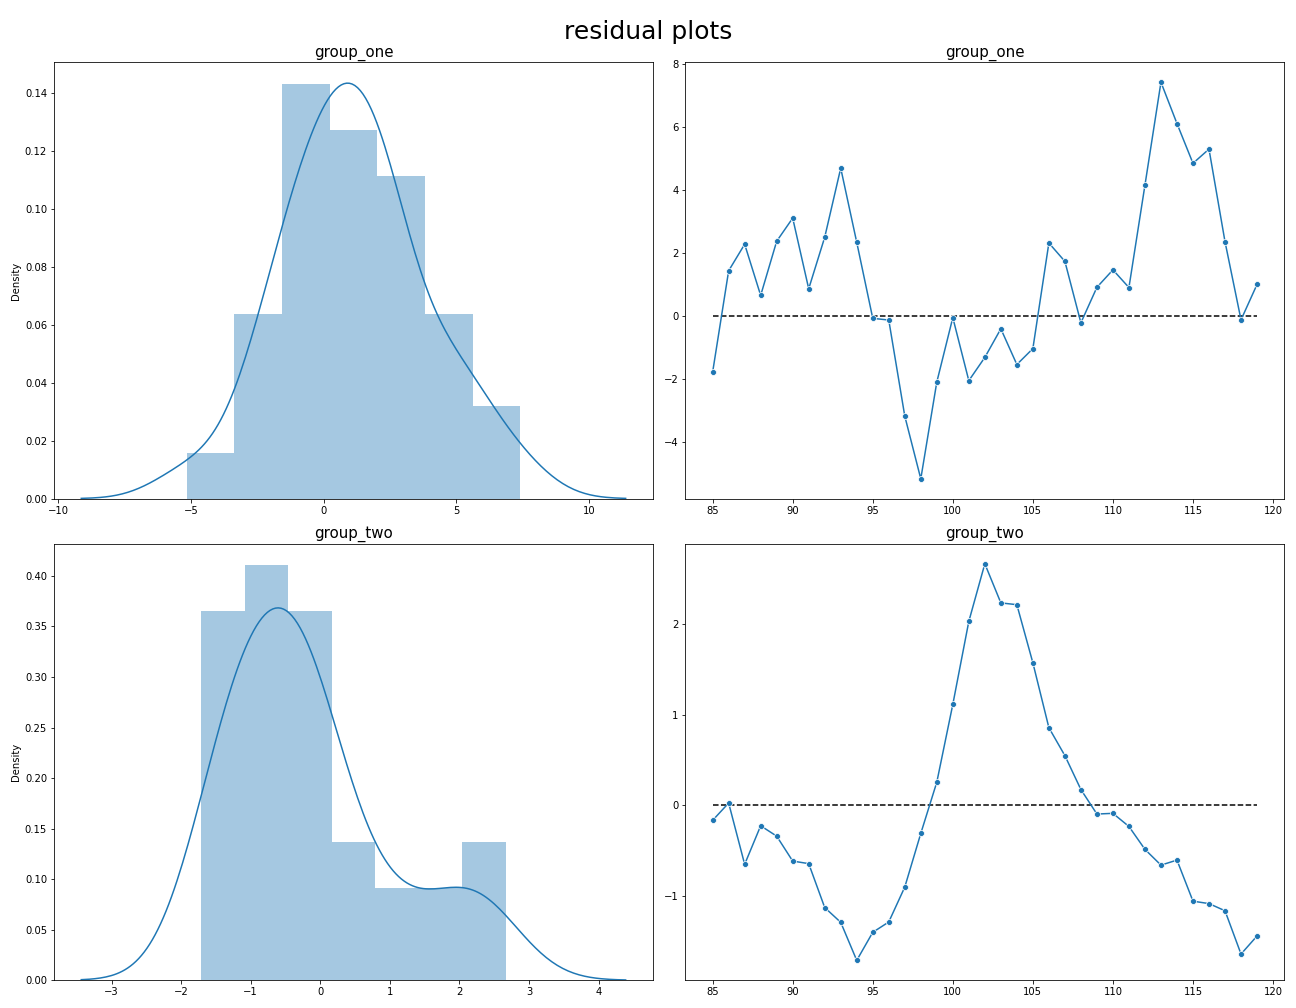
\includegraphics[width = 0.45 \textwidth]{../plots/ex1_third_residual_plots_all.png}}
    \subfigure[Third Plot]{%
        \label{fig:supfigure3}
        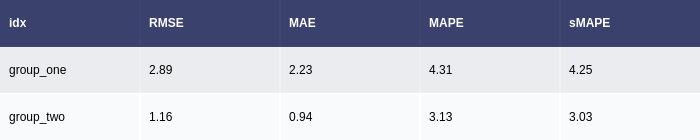
\includegraphics[width = 0.75 \textwidth]{../plots/ex1_third_get_errors.png}}
    \quad
    \caption{Predictions in one and 2 groups}
\end{figure}

\subsection{Example 2}

\begin{figure}[H]
    \centerline{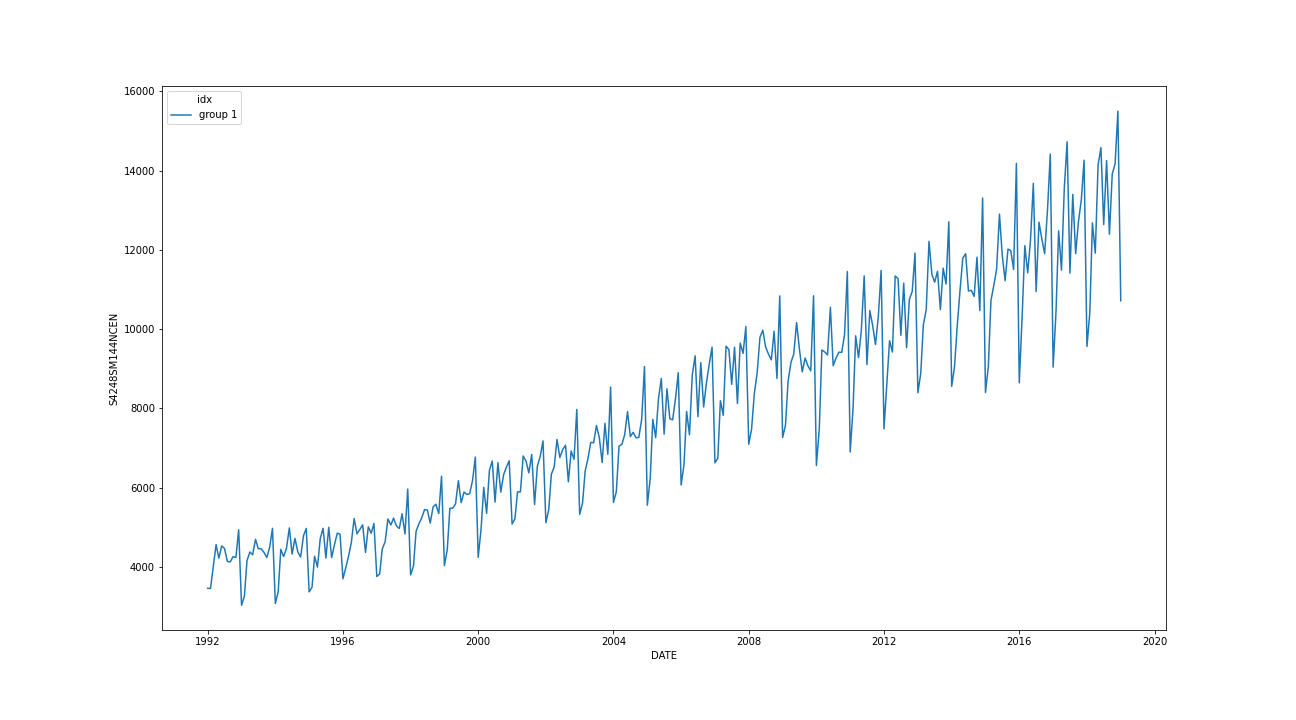
\includegraphics[scale = 0.45]{../plots/ex2_plot_data.png}}
    \caption{Lineplot of the data}
\end{figure}

\begin{figure}[H]
    \centering
    \subfigure[First plot]{%
        \label{fig:supfigure1}
        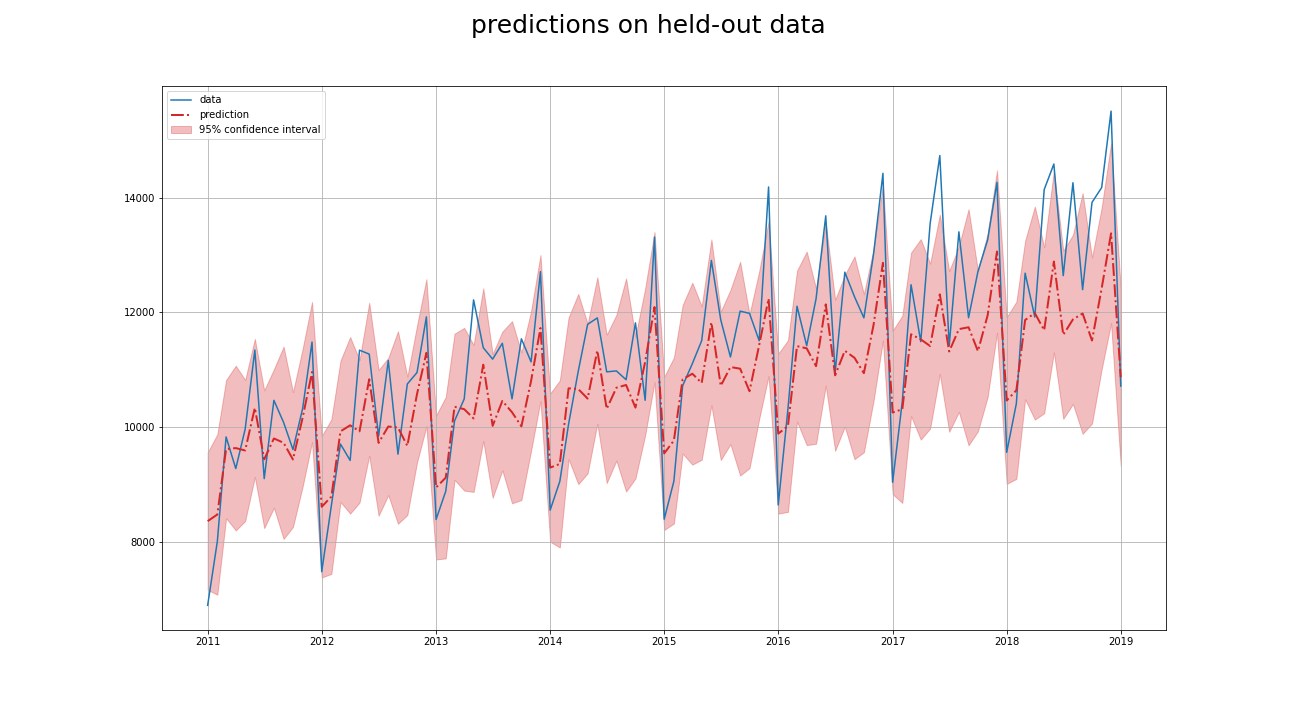
\includegraphics[width = 0.75 \textwidth]{../plots/ex2_plot_predict_idx_full.png}}
    \quad
    \subfigure[Second plot]{%
        \label{fig:supfigure2}
        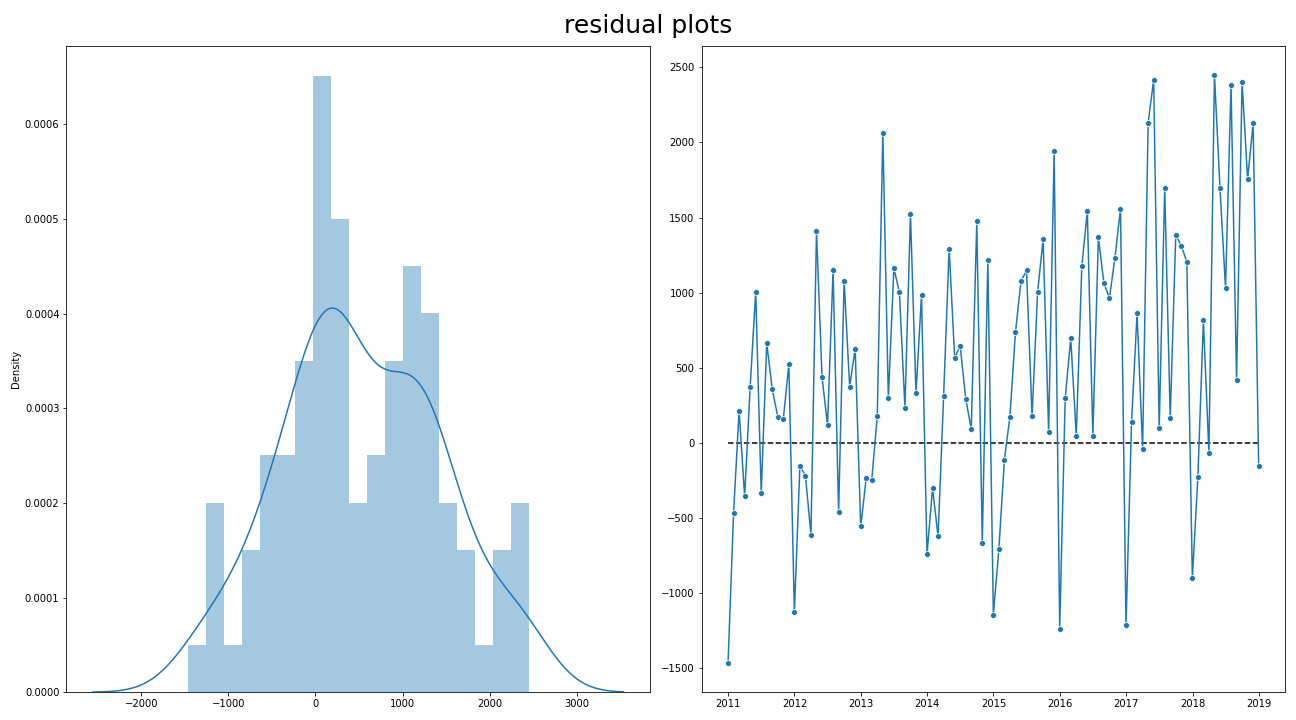
\includegraphics[width = 0.75 \textwidth]{../plots/ex2_plot_residuals_full.png}}
    \subfigure[Third Plot]{%
        \label{fig:supfigure3}
        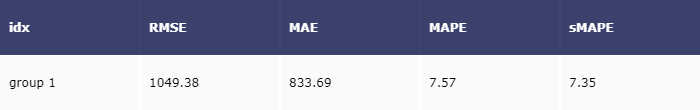
\includegraphics[width = 0.75 \textwidth]{../plots/ex2_get_errors_full.png}}
    \quad
    \caption{Predictions in one and 2 groups}
\end{figure}

\begin{figure}[H]
    \centering
    \subfigure[First plot]{%
        \label{fig:supfigure1}
        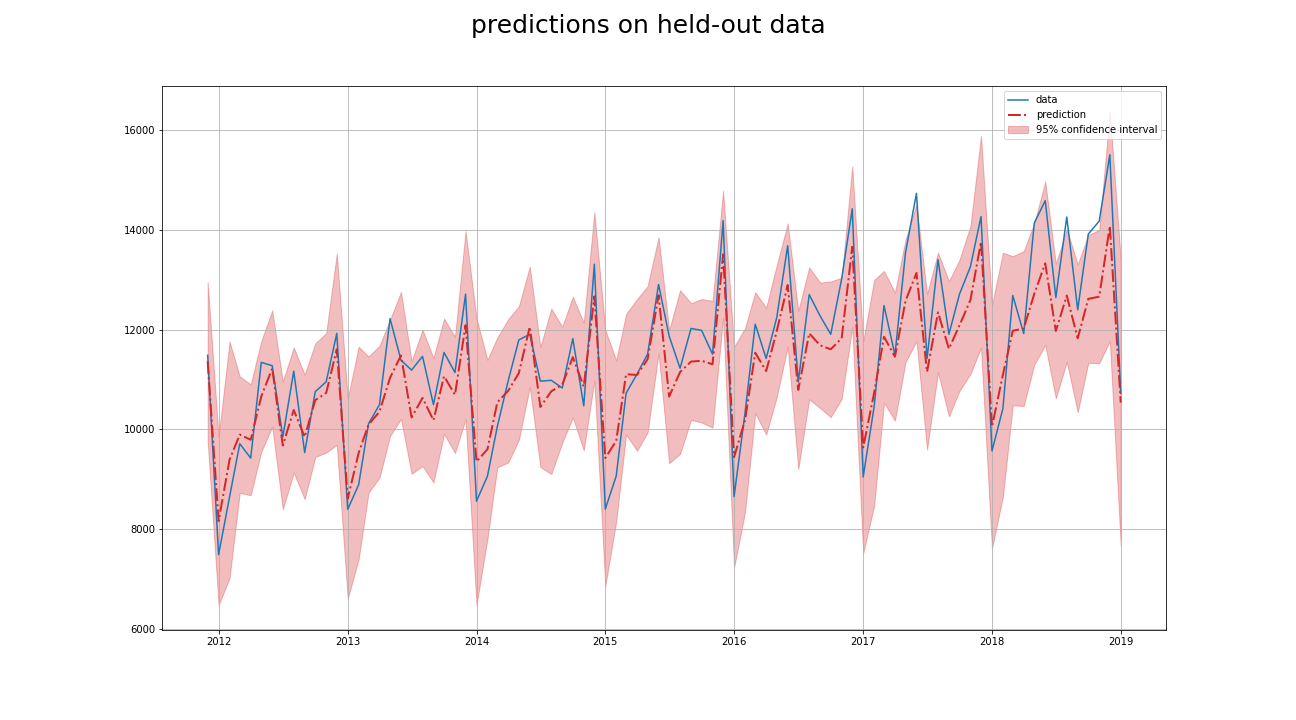
\includegraphics[width = 0.75 \textwidth]{../plots/ex2_plot_predict_idx_crop.png}}
    \quad
    \subfigure[Second plot]{%
        \label{fig:supfigure2}
        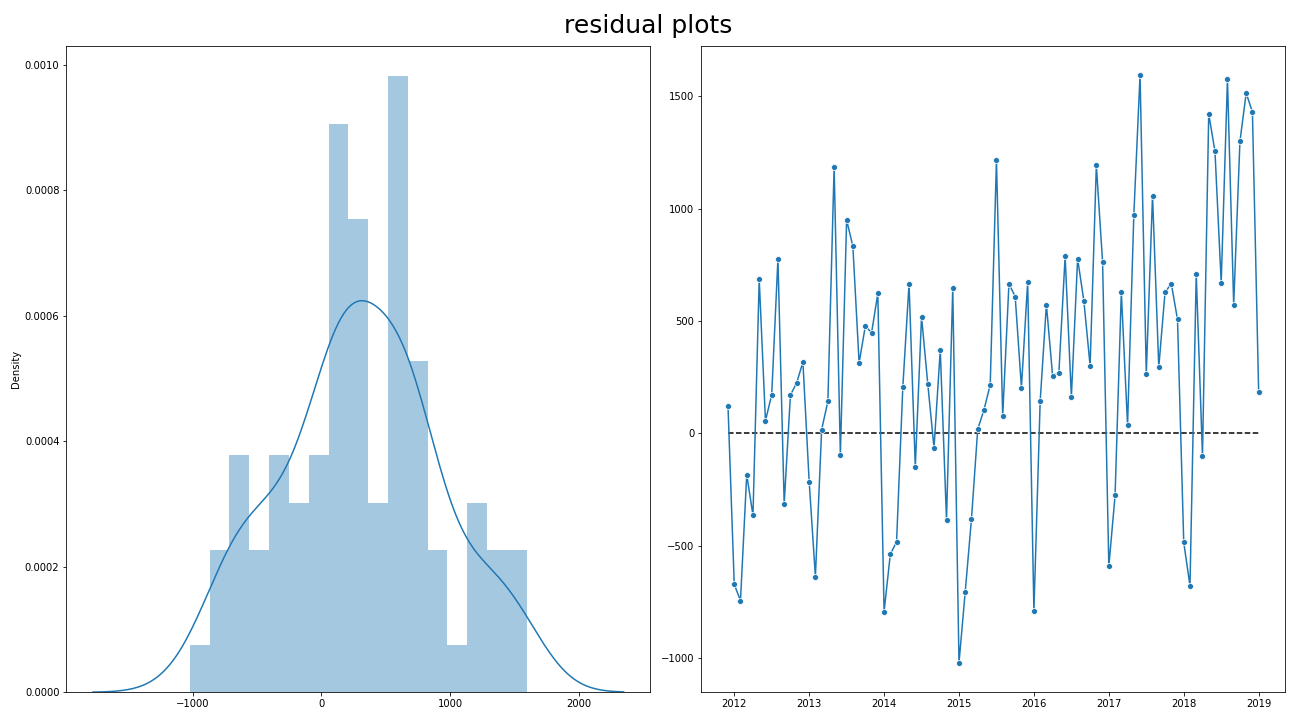
\includegraphics[width = 0.75 \textwidth]{../plots/ex2_plot_residuals_crop.png}}
    \subfigure[Third Plot]{%
        \label{fig:supfigure3}
        
\includegraphics[width = 0.75 \textwidth]{../plots/ex2_get_errors_crop.png}}
    \quad
    \caption{Predictions in one and 2 groups}
\end{figure}

\subsection{Example 3}

\begin{figure}[H]
    \centerline{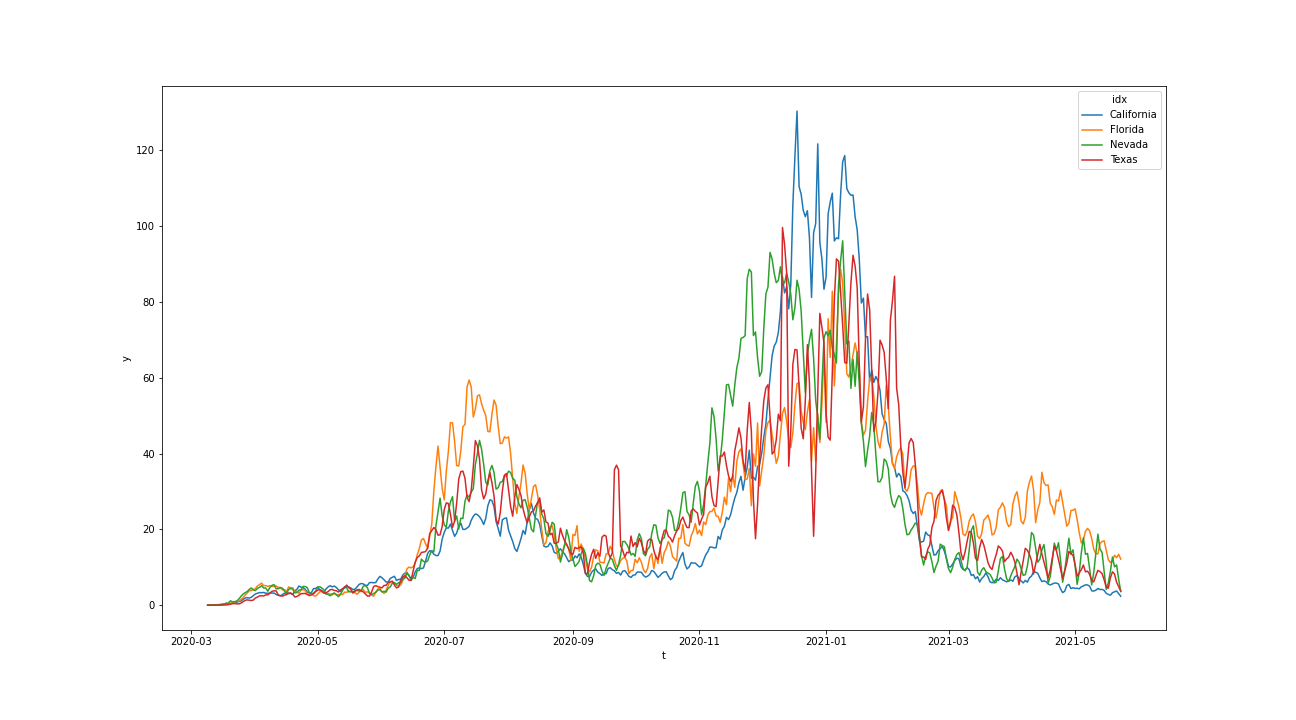
\includegraphics[scale = 0.45]{../plots/ex3_raw_data.png}}
    \caption{Lineplot of the data}
\end{figure}

\begin{figure}[H]
    \centering
    \subfigure[First plot]{%
        \label{fig:supfigure1}
        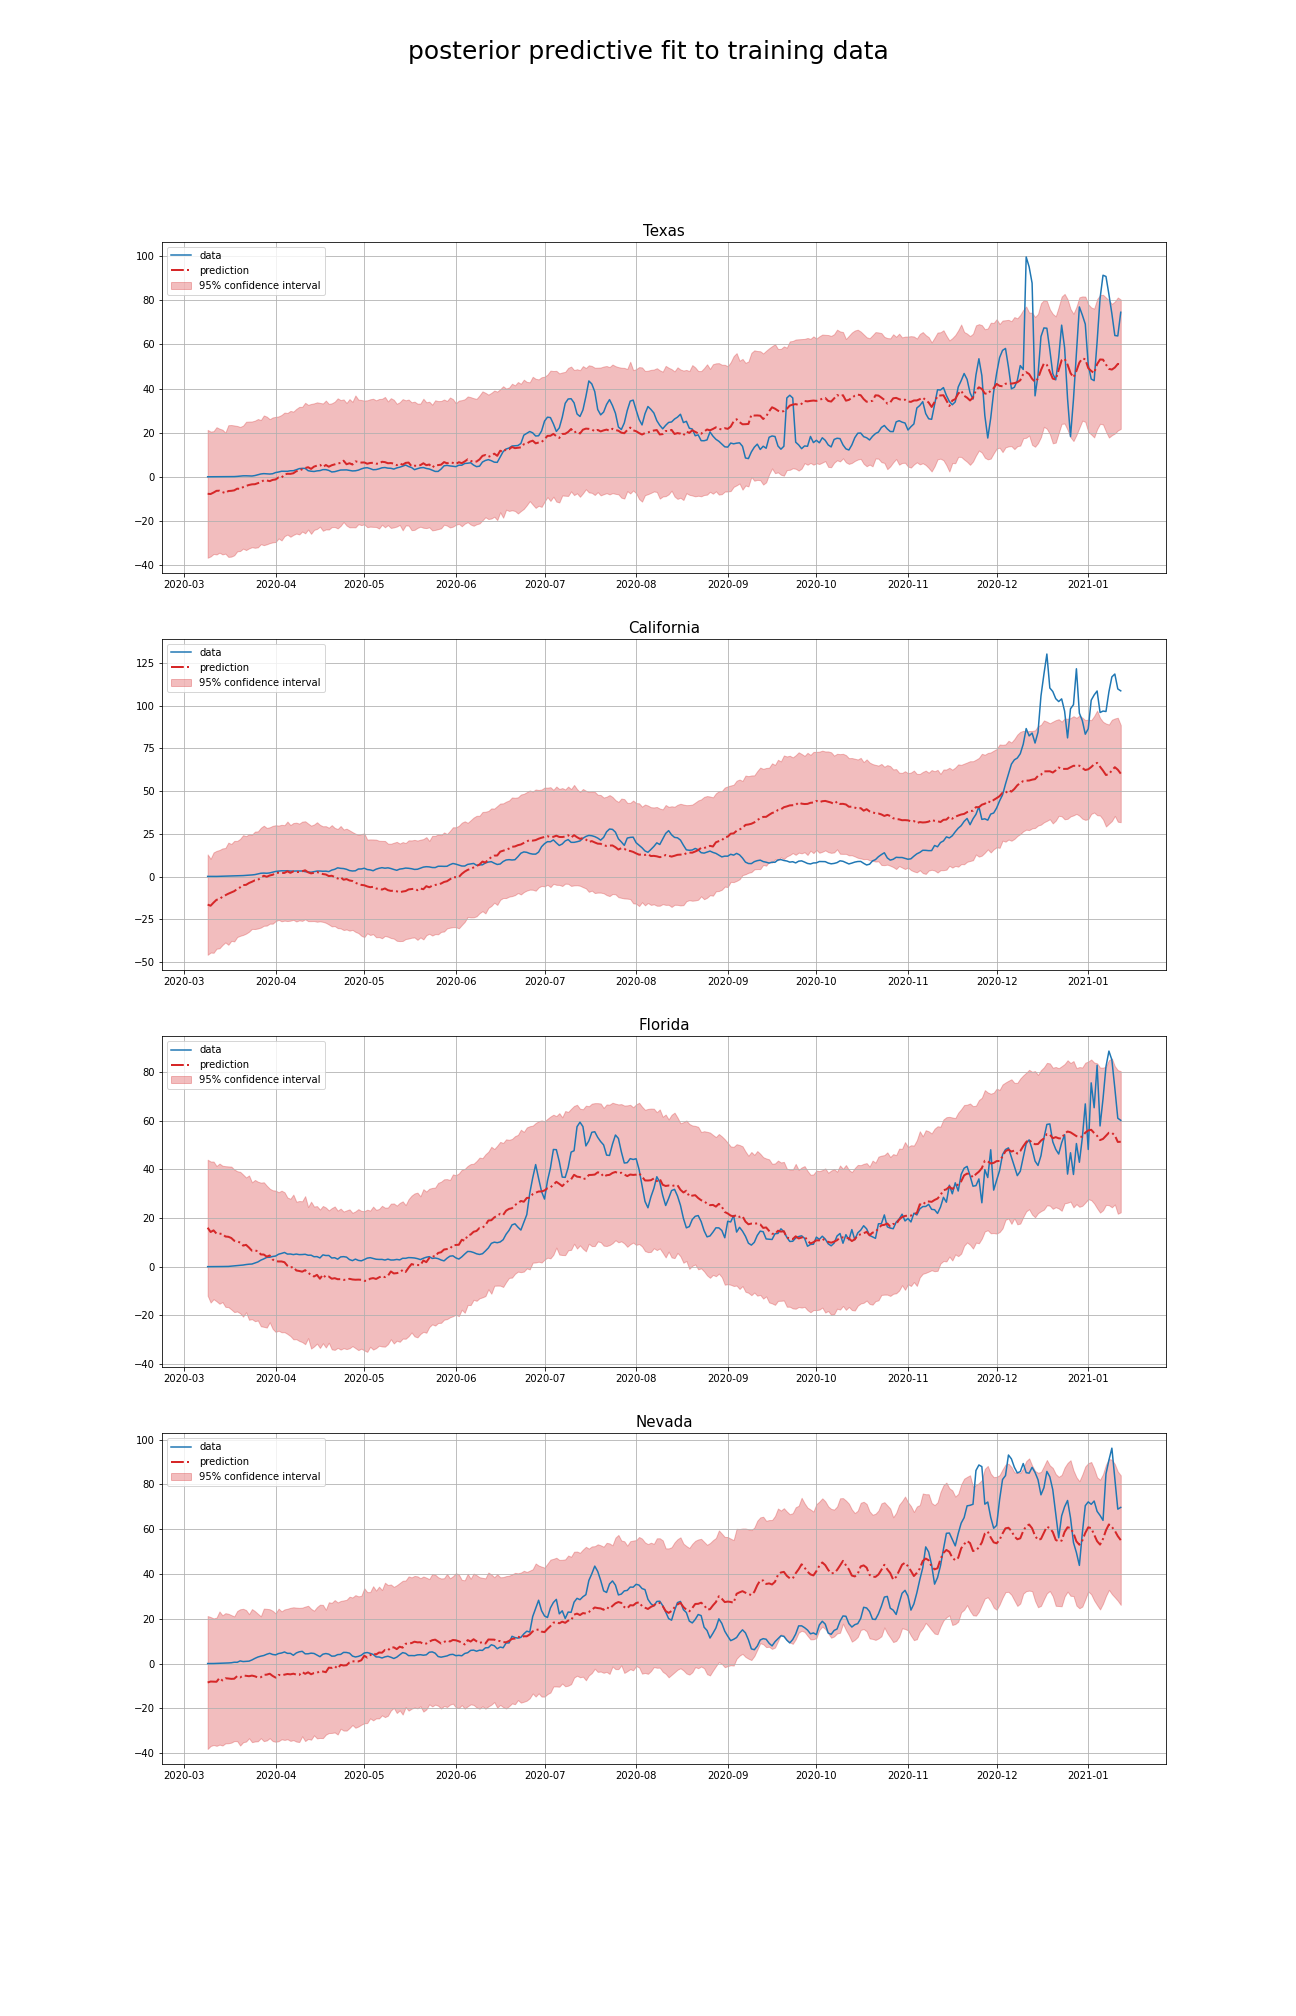
\includegraphics[width = 0.45 \textwidth]{../plots/ex3_plot_fit_idx.png}}
    \quad
    \subfigure[Second plot]{%
        \label{fig:supfigure2}
        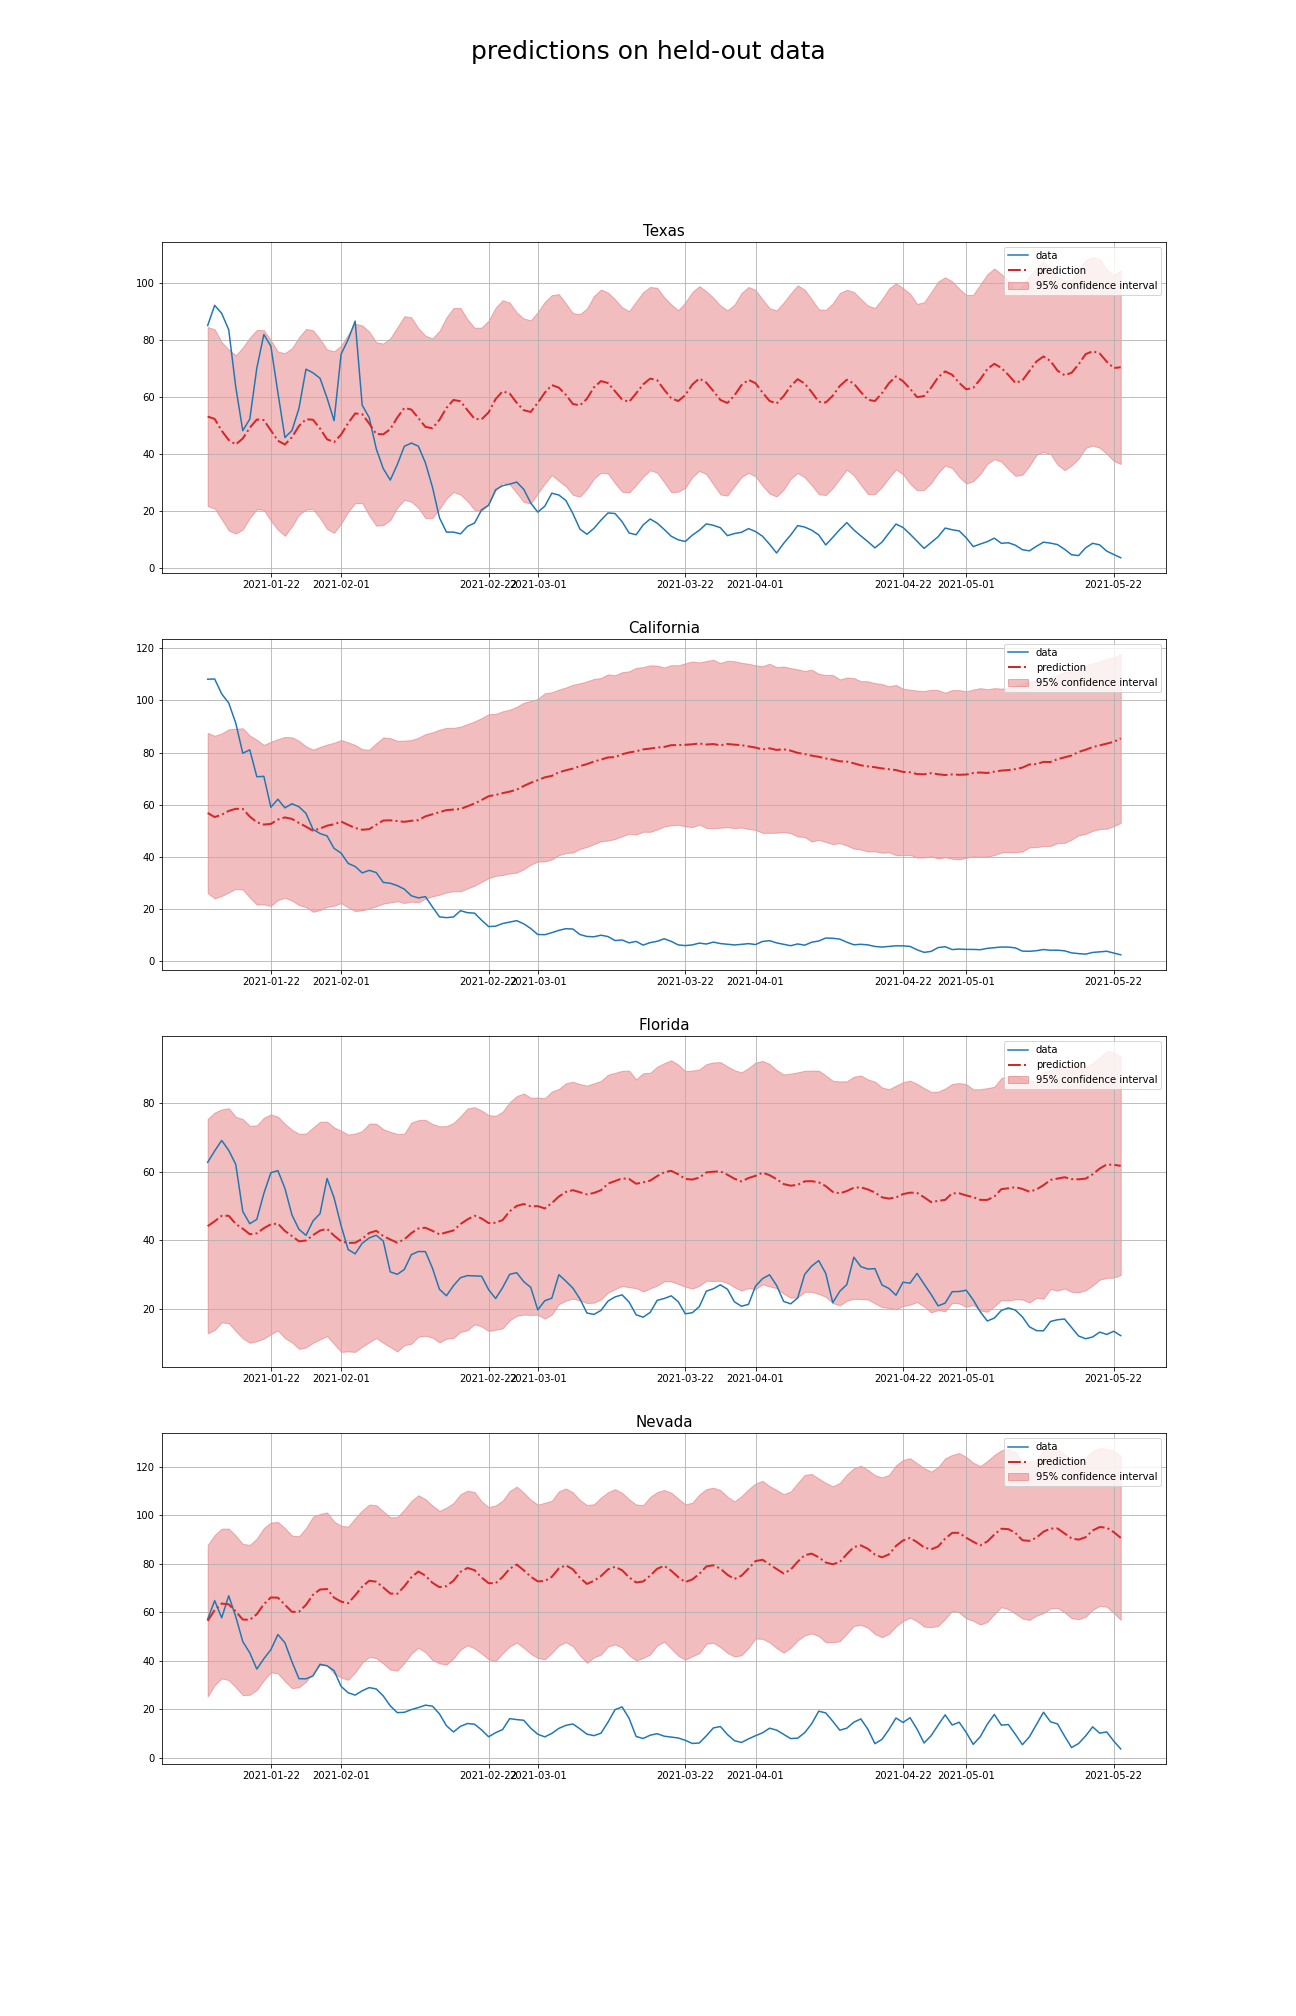
\includegraphics[width = 0.45 \textwidth]{../plots/ex3_plot_predict_idx.png}}
    \caption{Predictions in one and 2 groups}
\end{figure}

\section{Limitations and future work}

\subsection{The Goal of PyCipio}

\subsection{Flexibility}

\subsection{Hierarchical}

\subsection{Prediction on unseen data set}

\bibliographystyle{apacite}

\bibliography{../Referencer}

\end{document}